\documentclass{article}
\usepackage{graphicx}
\usepackage[style=ieee]{biblatex} % Set the reference style to IEEE
\usepackage{xcolor}
\usepackage{hyperref}
\usepackage{titletoc}

\definecolor{mygreen}{RGB}{0,128,0}

\usepackage{array} % For customizing the table
\usepackage{booktabs} % For better quality horizontal lines
\usepackage{graphicx} % Package for including images
\usepackage{float}

% Define margins
\usepackage[margin=1in]{geometry}

\renewcommand{\contentsname}{\textcolor{mygreen}{Table of Contents}}

\begin{document}

\begin{titlepage}
    \centering
    % University logo
    % \includegraphics[width=0.24\textwidth]{logo.jpg}
    \par\vspace{2cm}

    % University name and course details
    {\Large \textbf{Institute of Aircraft Systems} \par}
    \vspace{0.5cm}
    {\large \textbf{University of Stuttgart} \par}
    \vspace{3cm}

    % Lab and activity details
    {\large \textbf{VVT Requirements Document} \par}
    {\large Capabilities and Limits of the XGEE Visualization Verification Pipeline \par}
    {\large  \par}
    \vspace{3cm}

    % Team members
    {\large \textbf{Team} \par}
    \vspace{0.5cm}
    \begin{tabular}{ll}
    Franz Köhler & st174932@stud.uni-stuttgart.de \\
    \end{tabular}
    \par\vspace{3cm}

    % Date
    {\large \today \par}
\end{titlepage}

\tableofcontents % Insert table of contents

\newpage % Page break to separate table of contents from document content

\section{Vertex too small}
\begin{figure}[H]
    \centering
    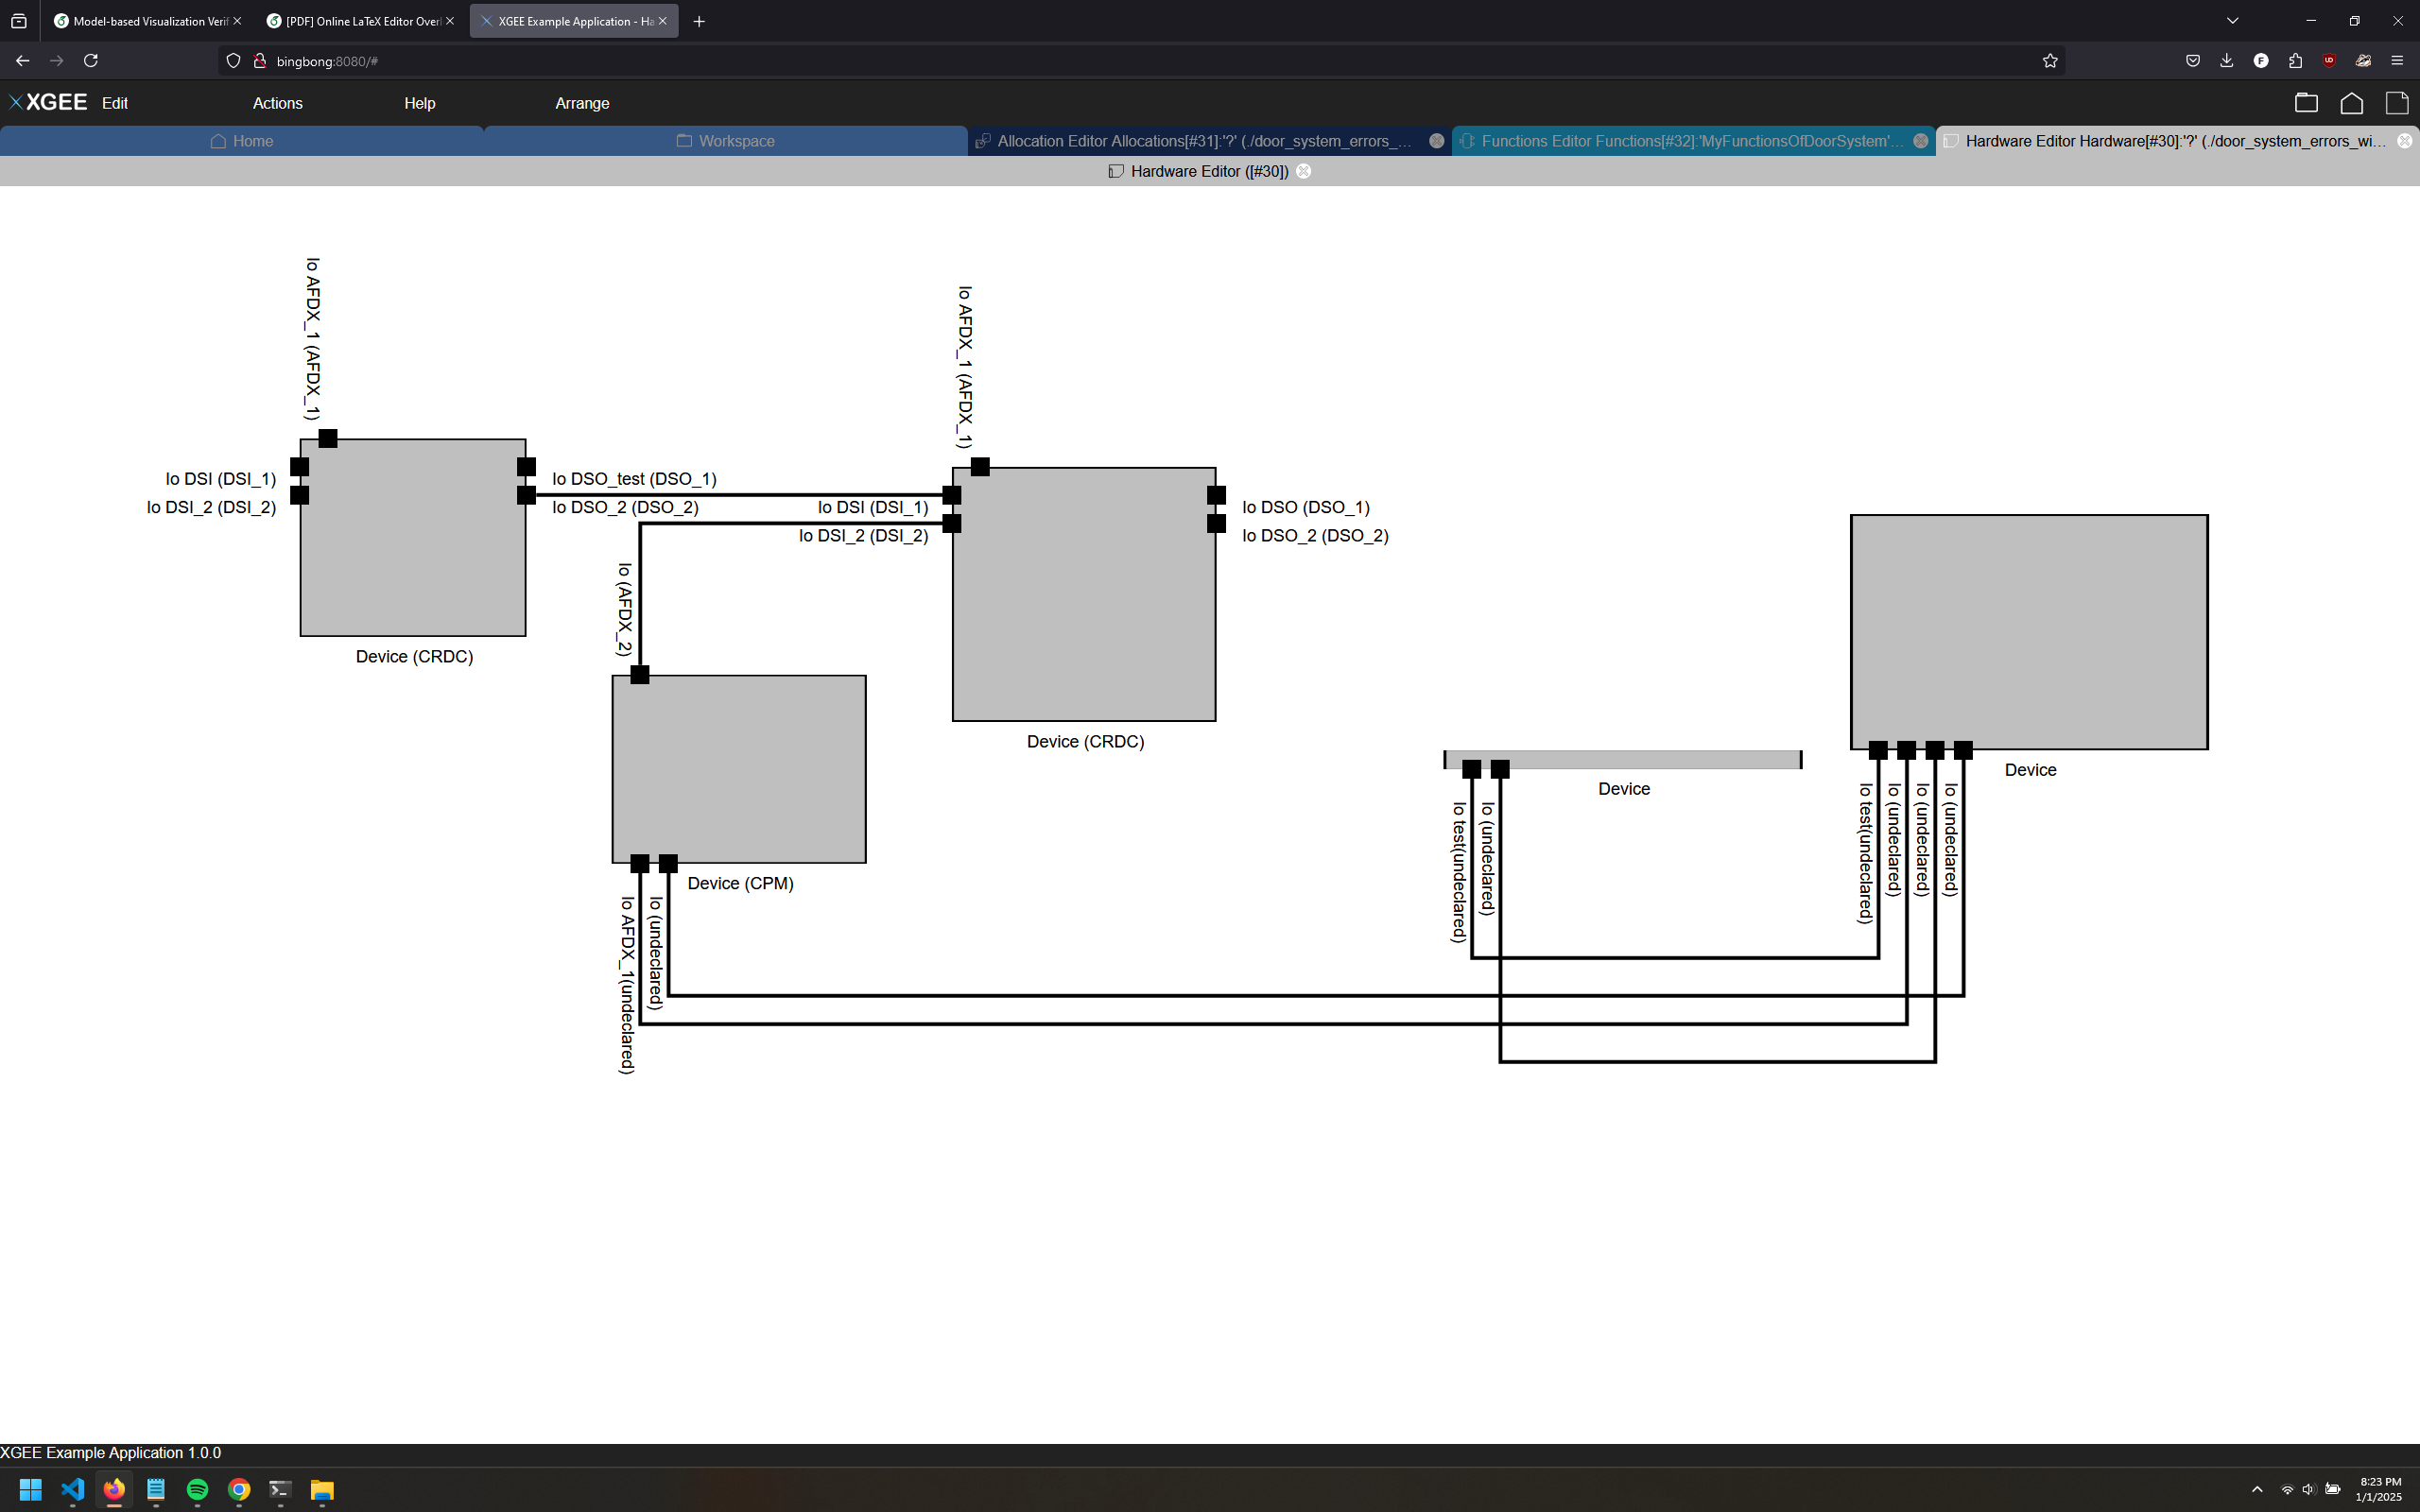
\includegraphics[width=0.9\textwidth]{images/vertex_too_small.png}
    \caption{Vertex too small}
\end{figure}
\newpage

\section{Vertex too large}
\begin{figure}[H]
    \centering
    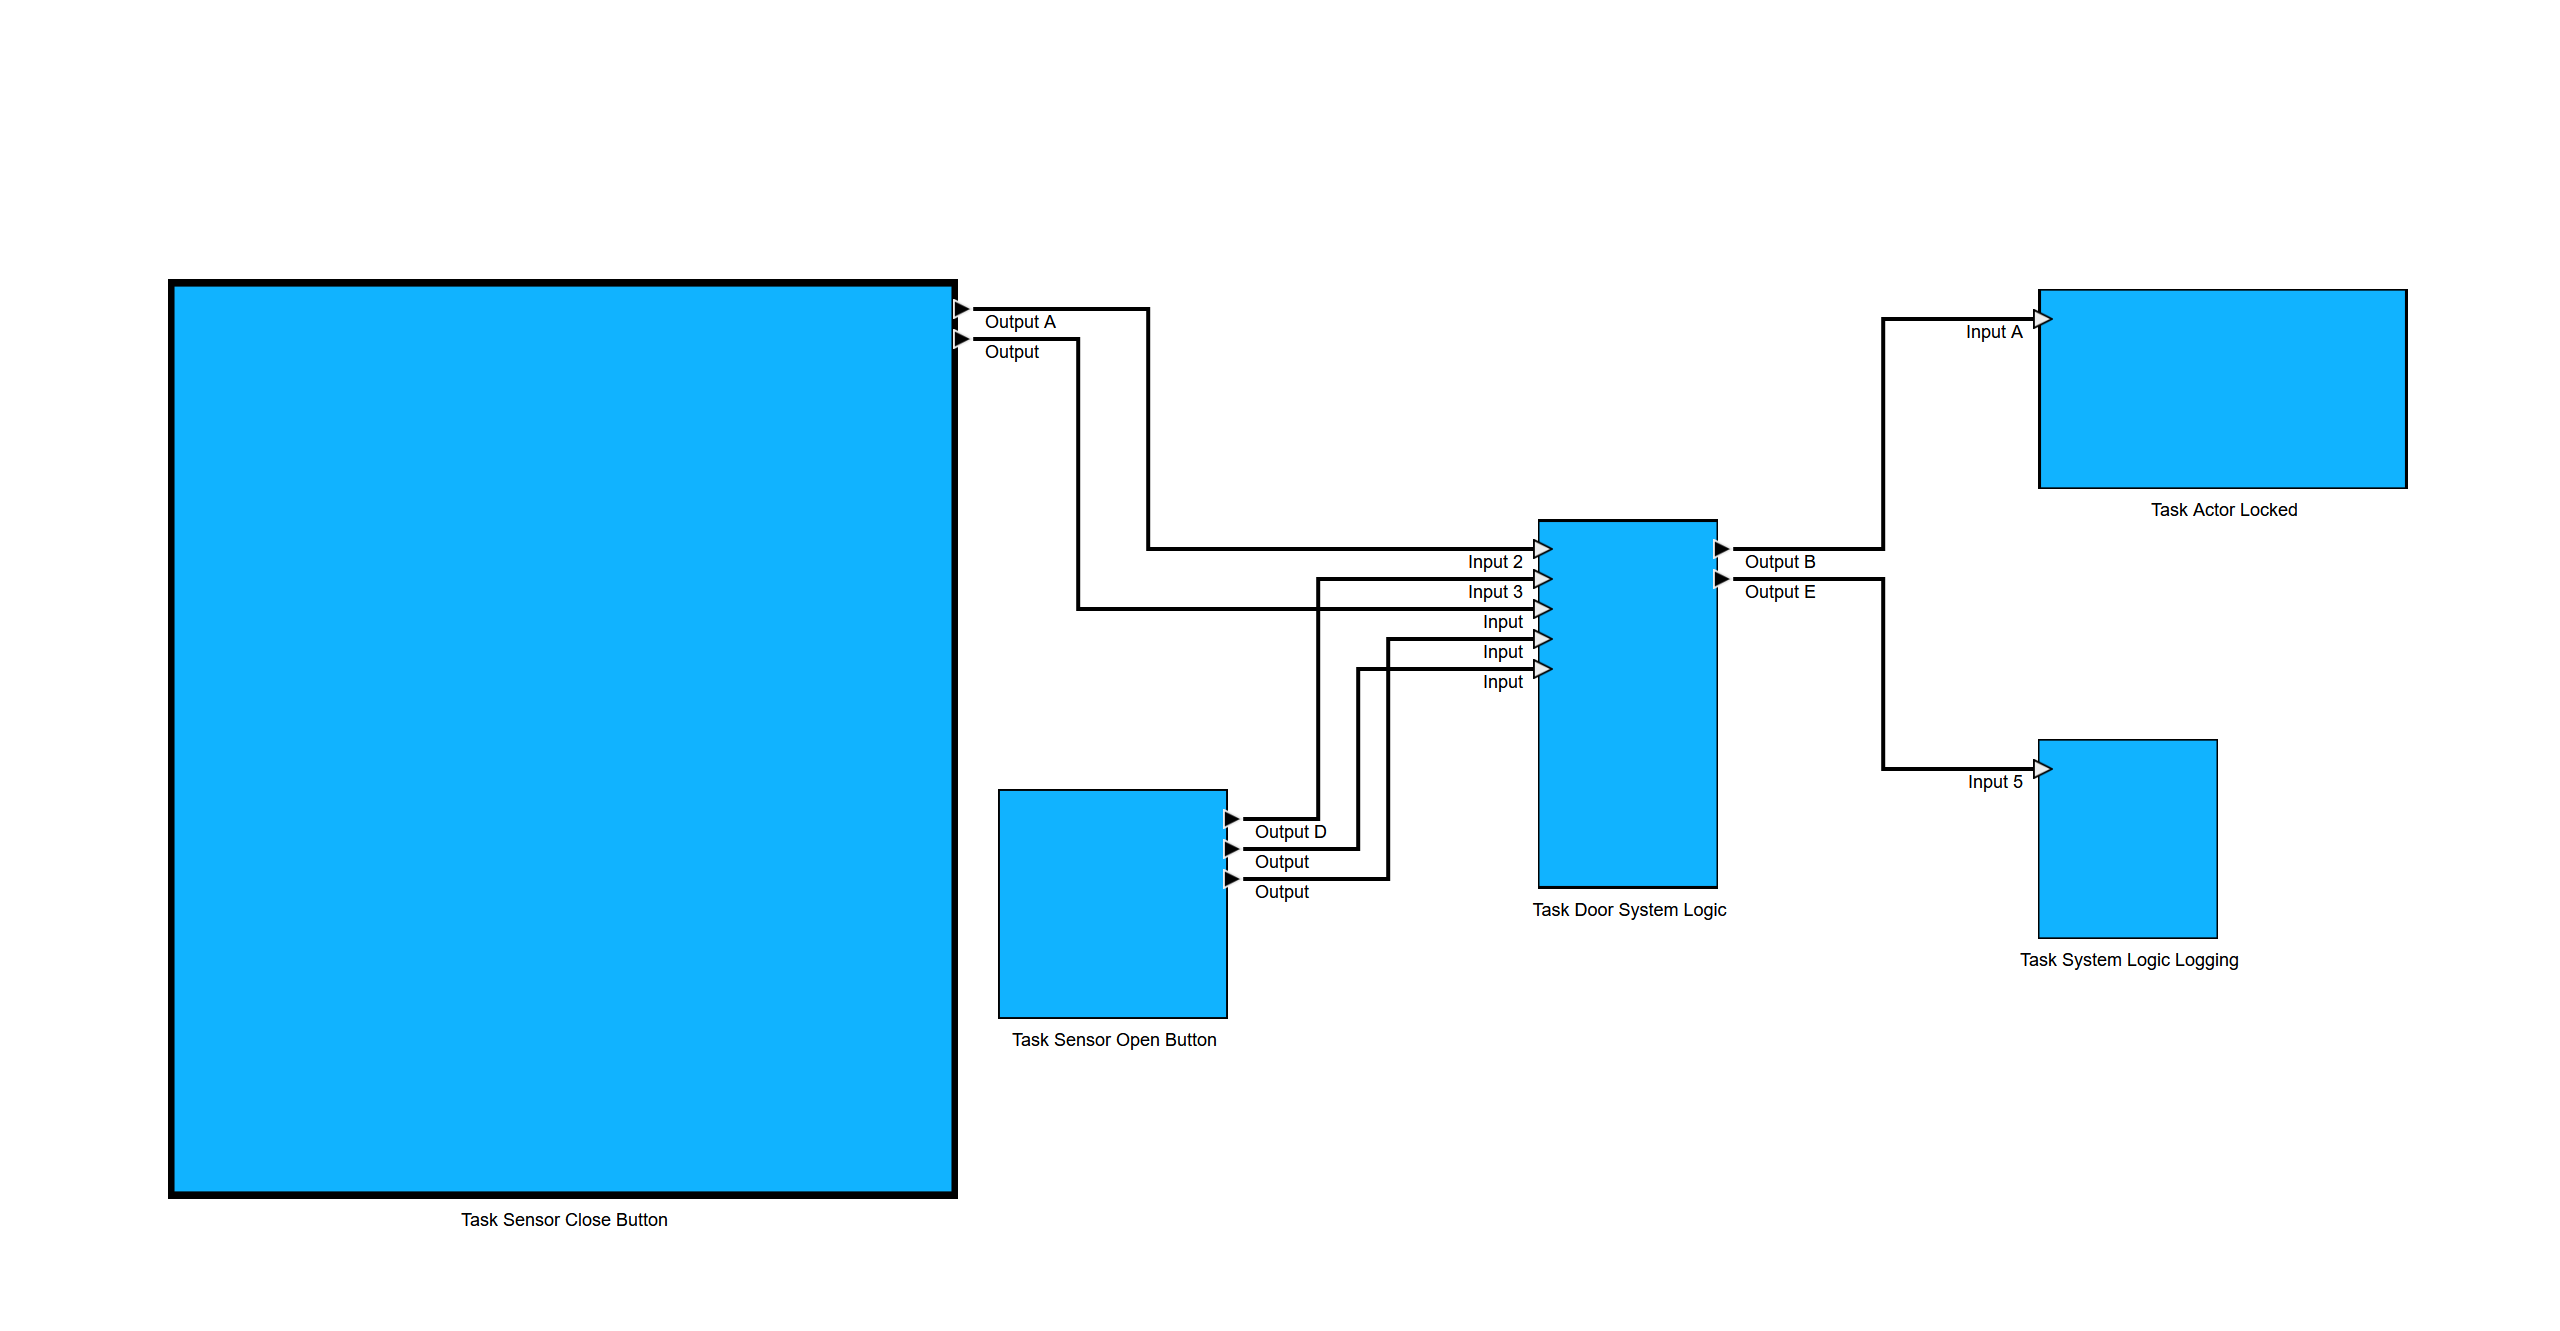
\includegraphics[width=0.9\textwidth]{images/vertex_too_large.png}
    \caption{Vertex too large}
\end{figure}
\newpage

\section{Vertex wrong color}
\begin{figure}[H]
    \centering
    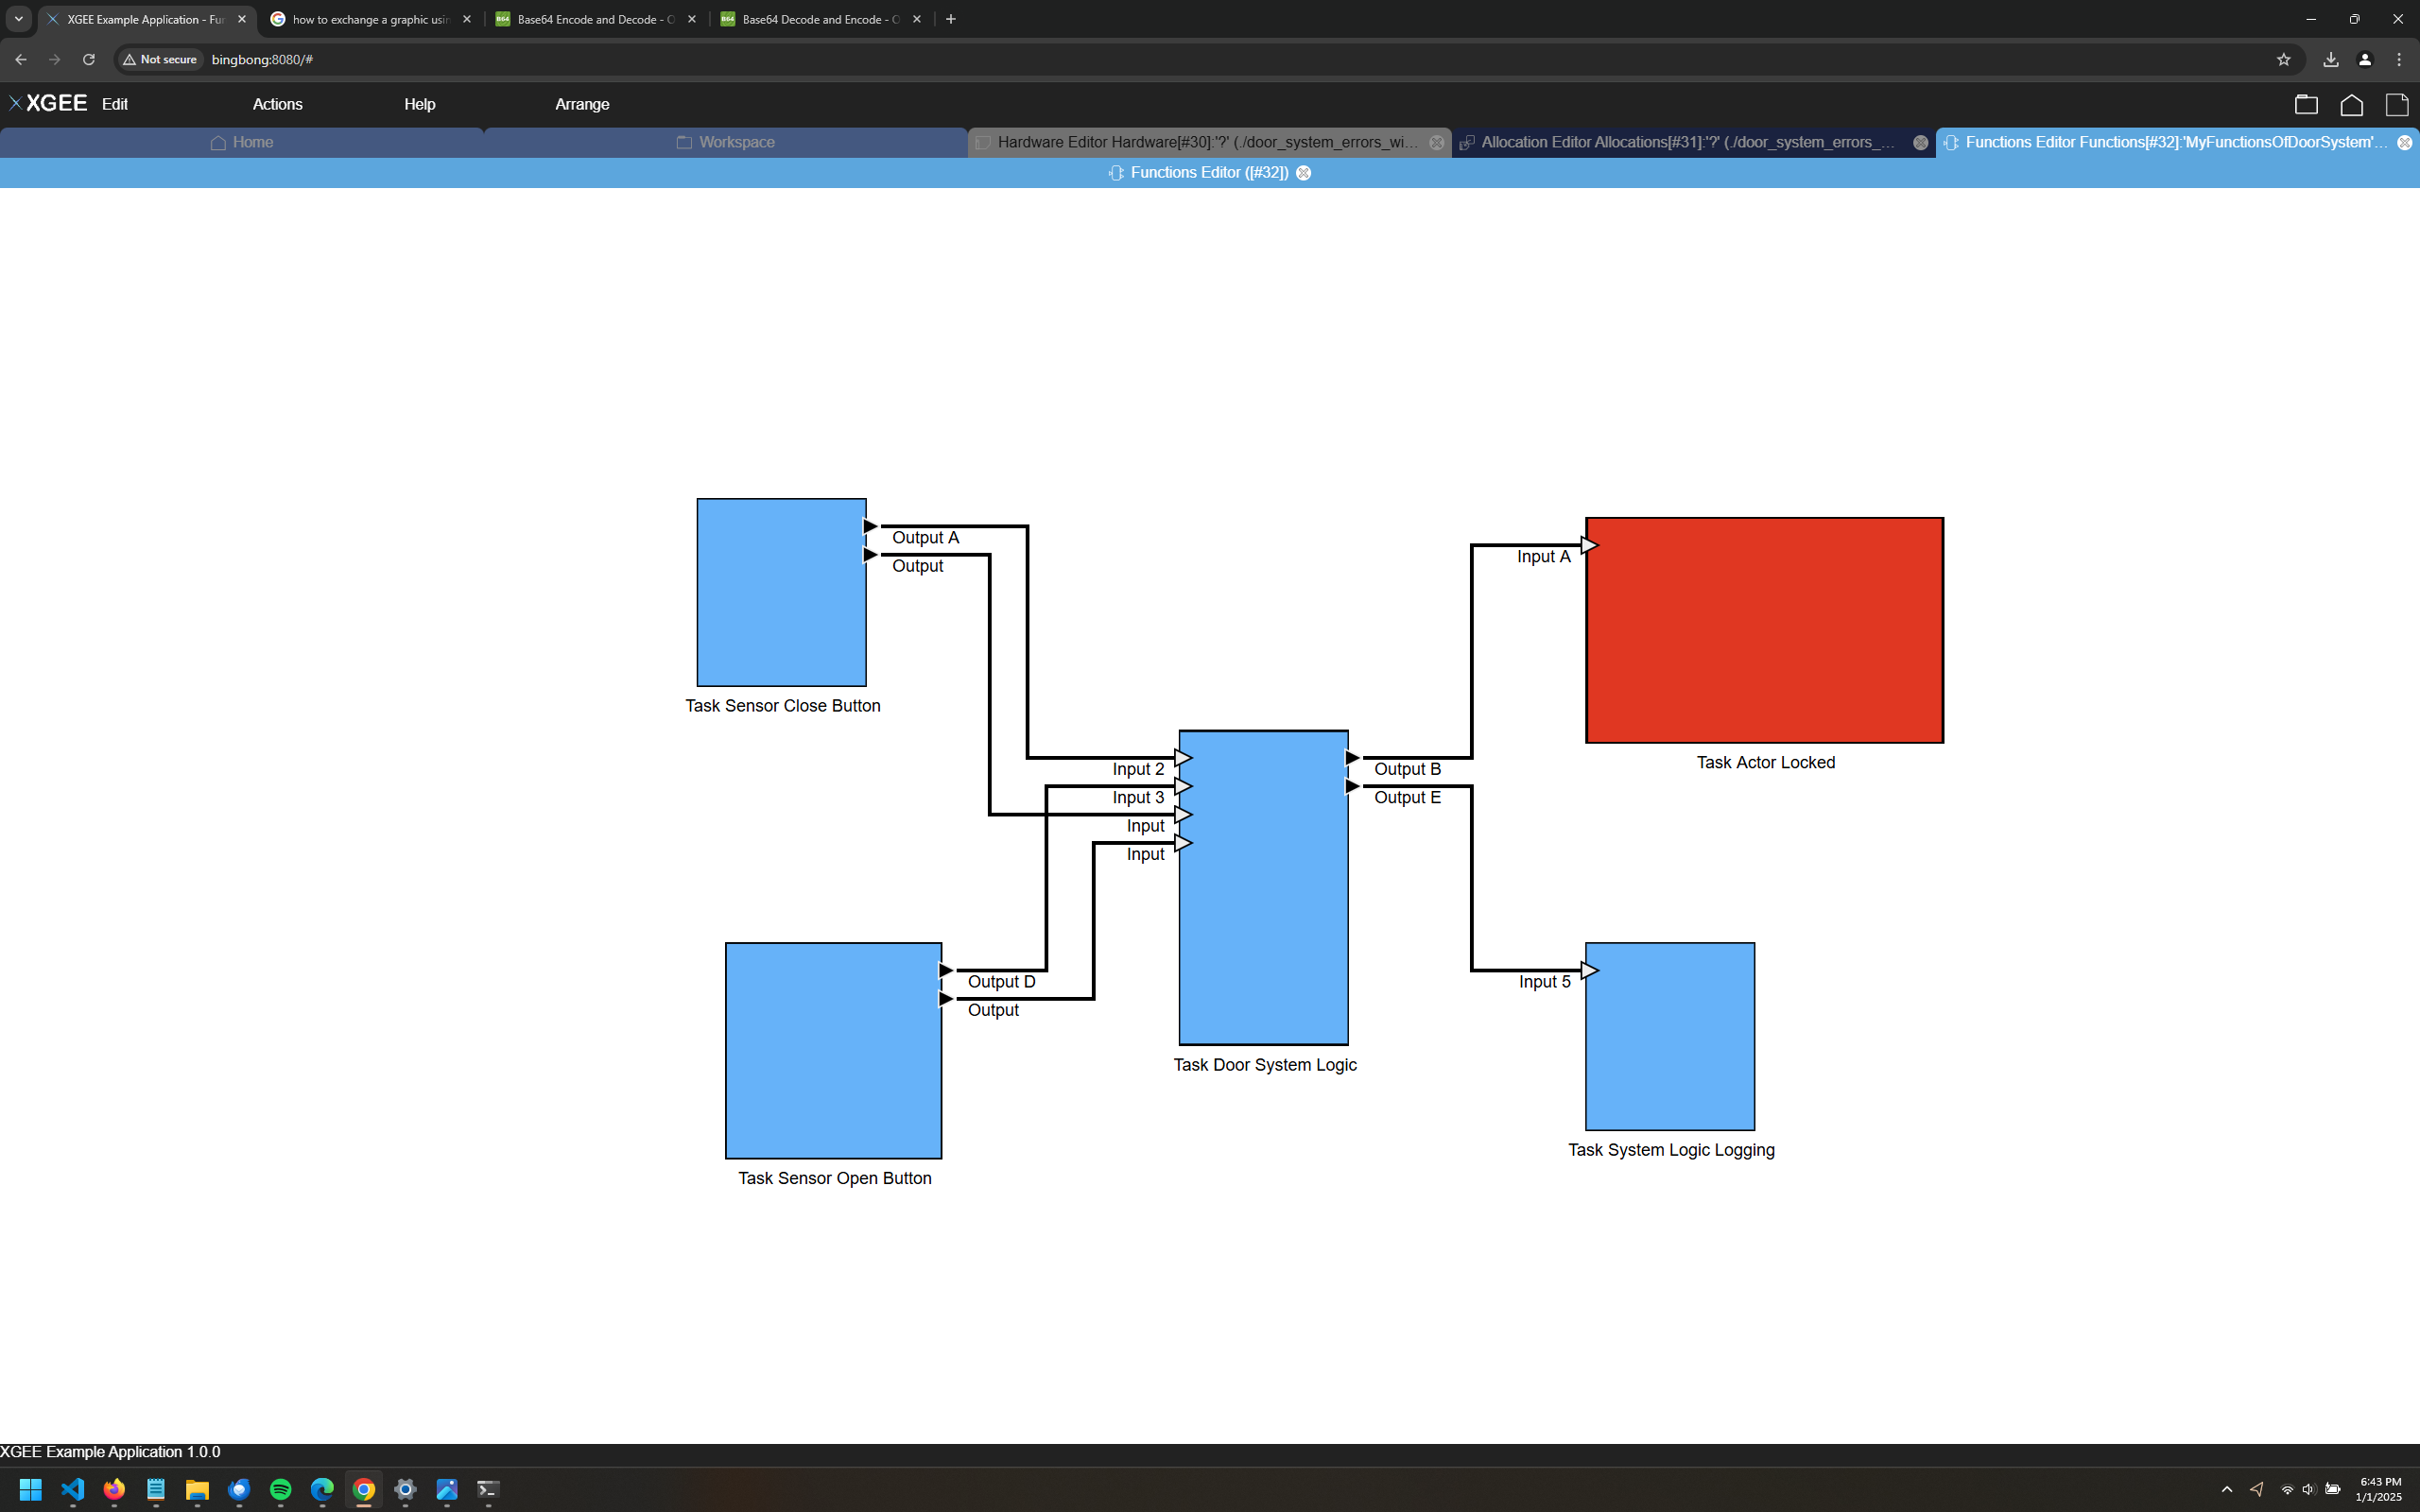
\includegraphics[width=0.9\textwidth]{images/vertex_wrong_color.png}
    \caption{Vertex wrong color}
\end{figure}
\newpage

\section{Vertex in wrong position}
\begin{figure}[H]
    \centering
    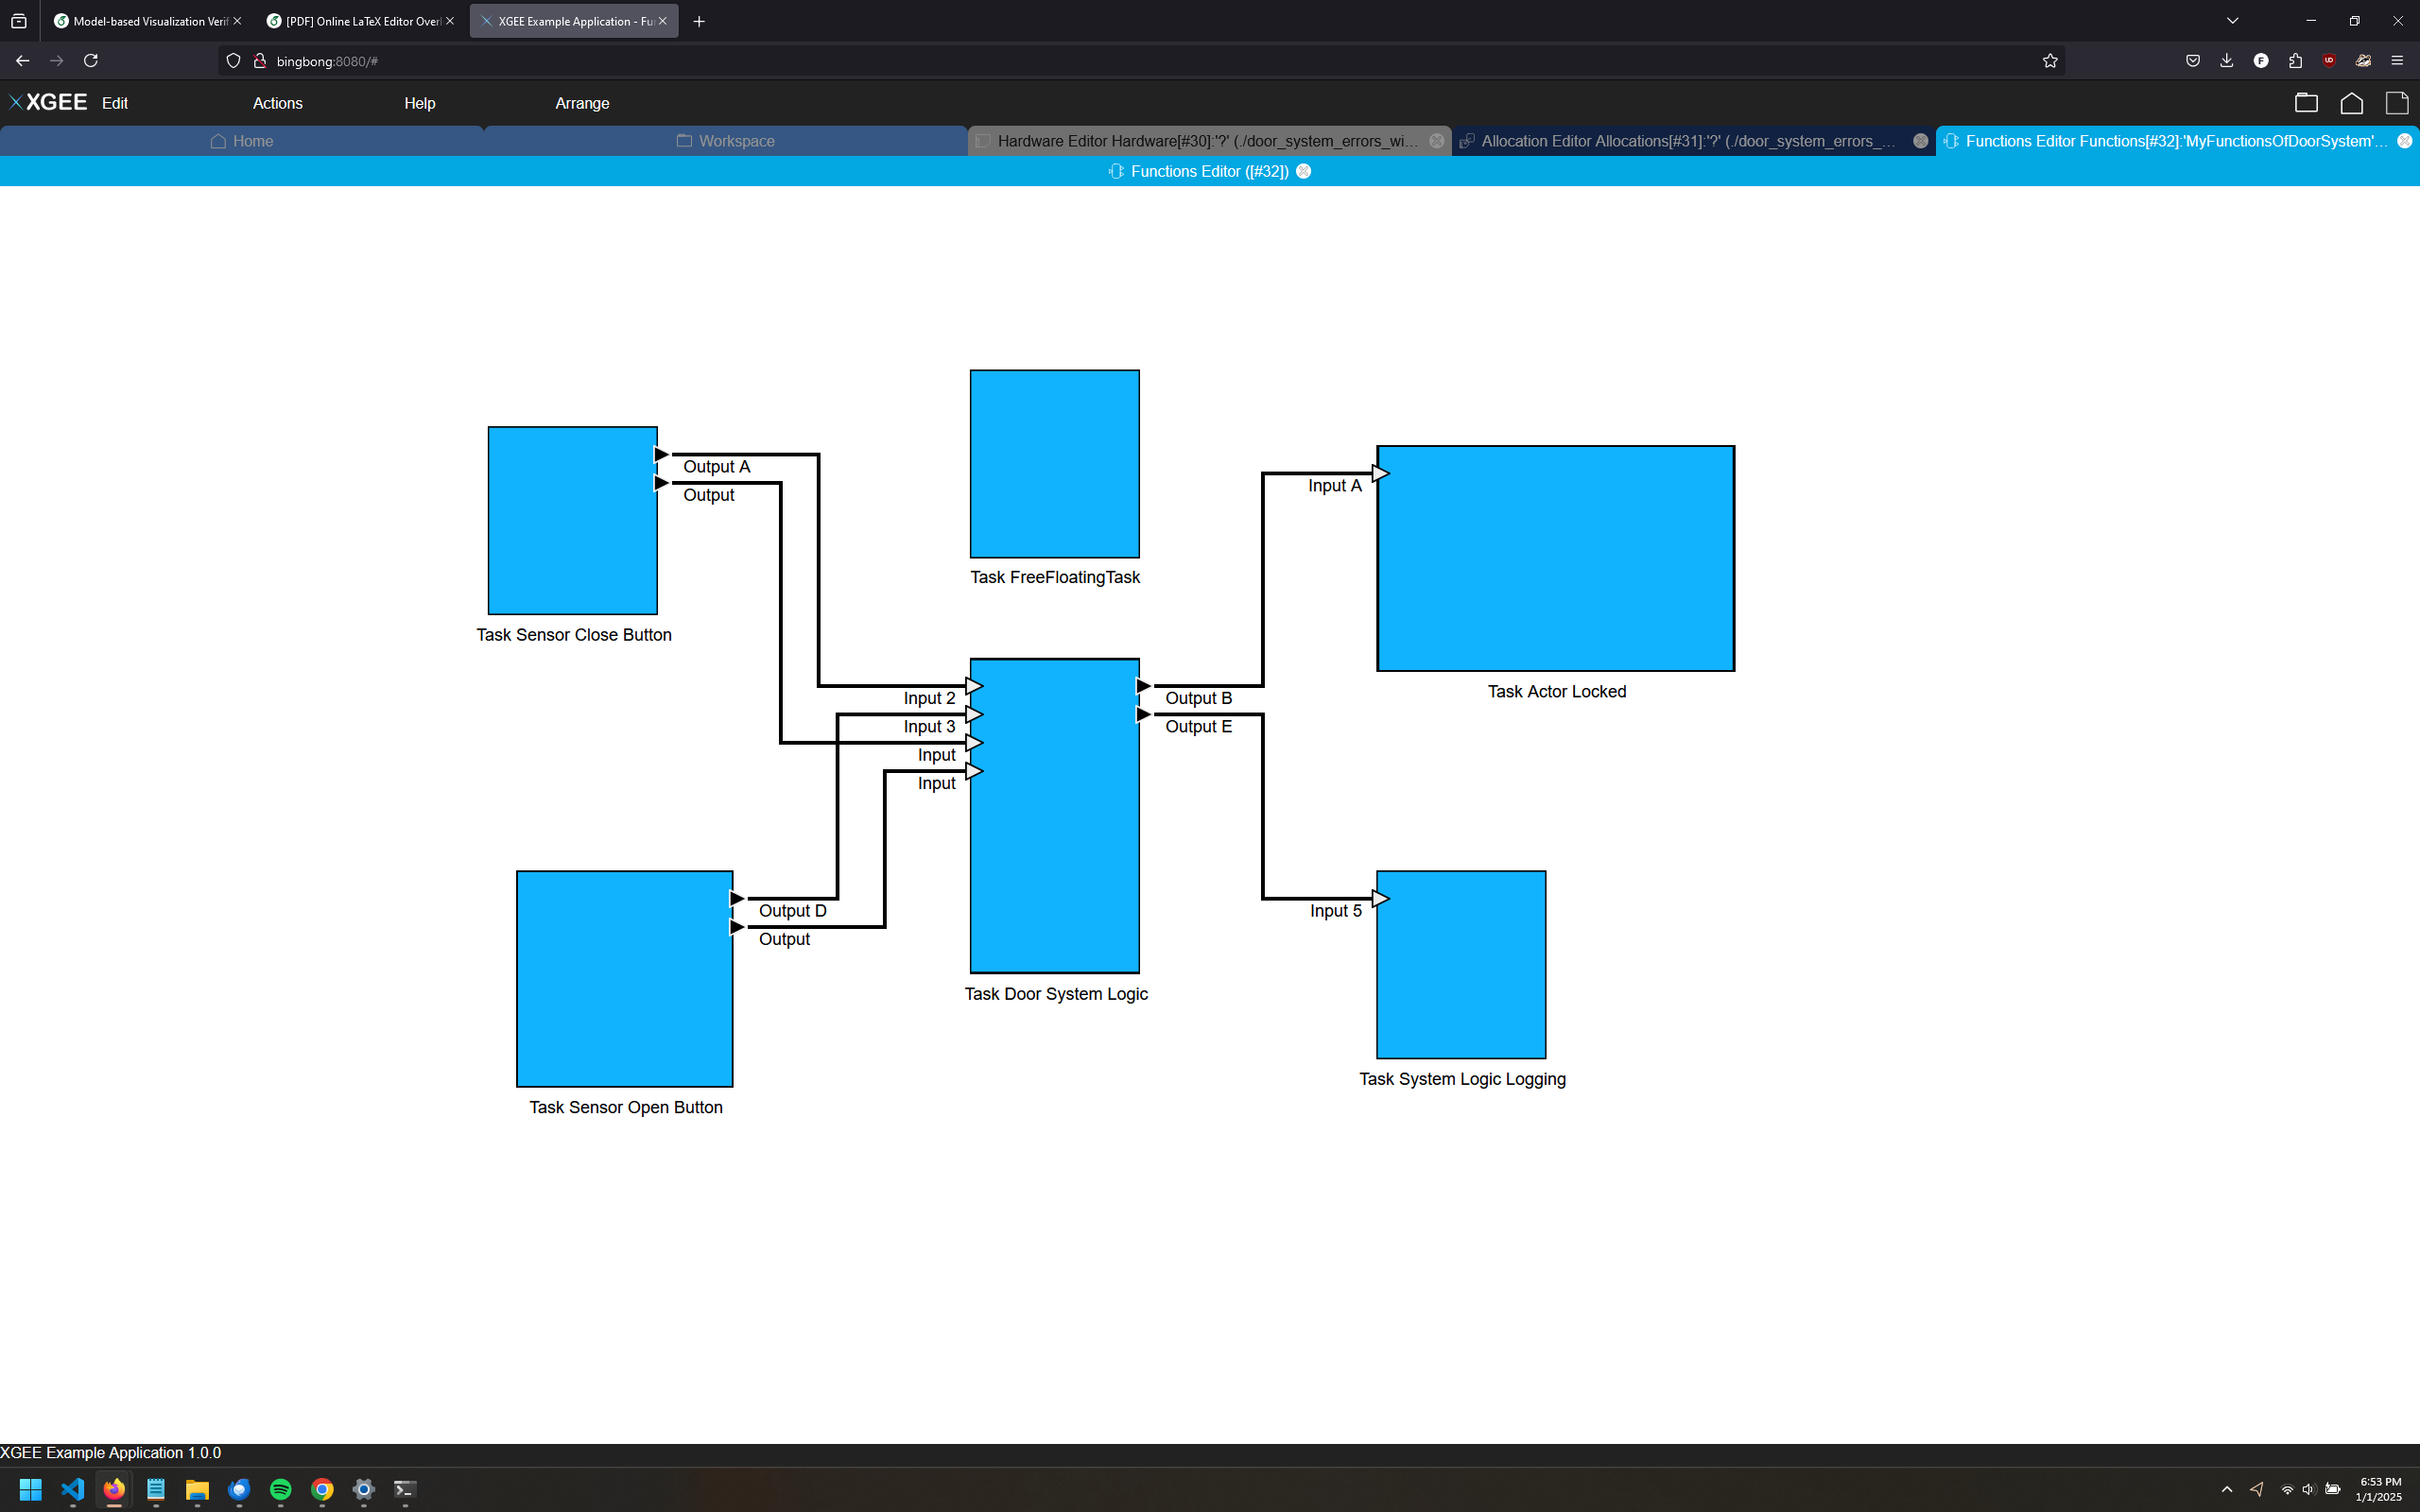
\includegraphics[width=0.9\textwidth]{images/vertex_in_wrong_position.png}
    \caption{Vertex in wrong position}
\end{figure}
\newpage

\section{Vertices too close to each other}
\begin{figure}[H]
    \centering
    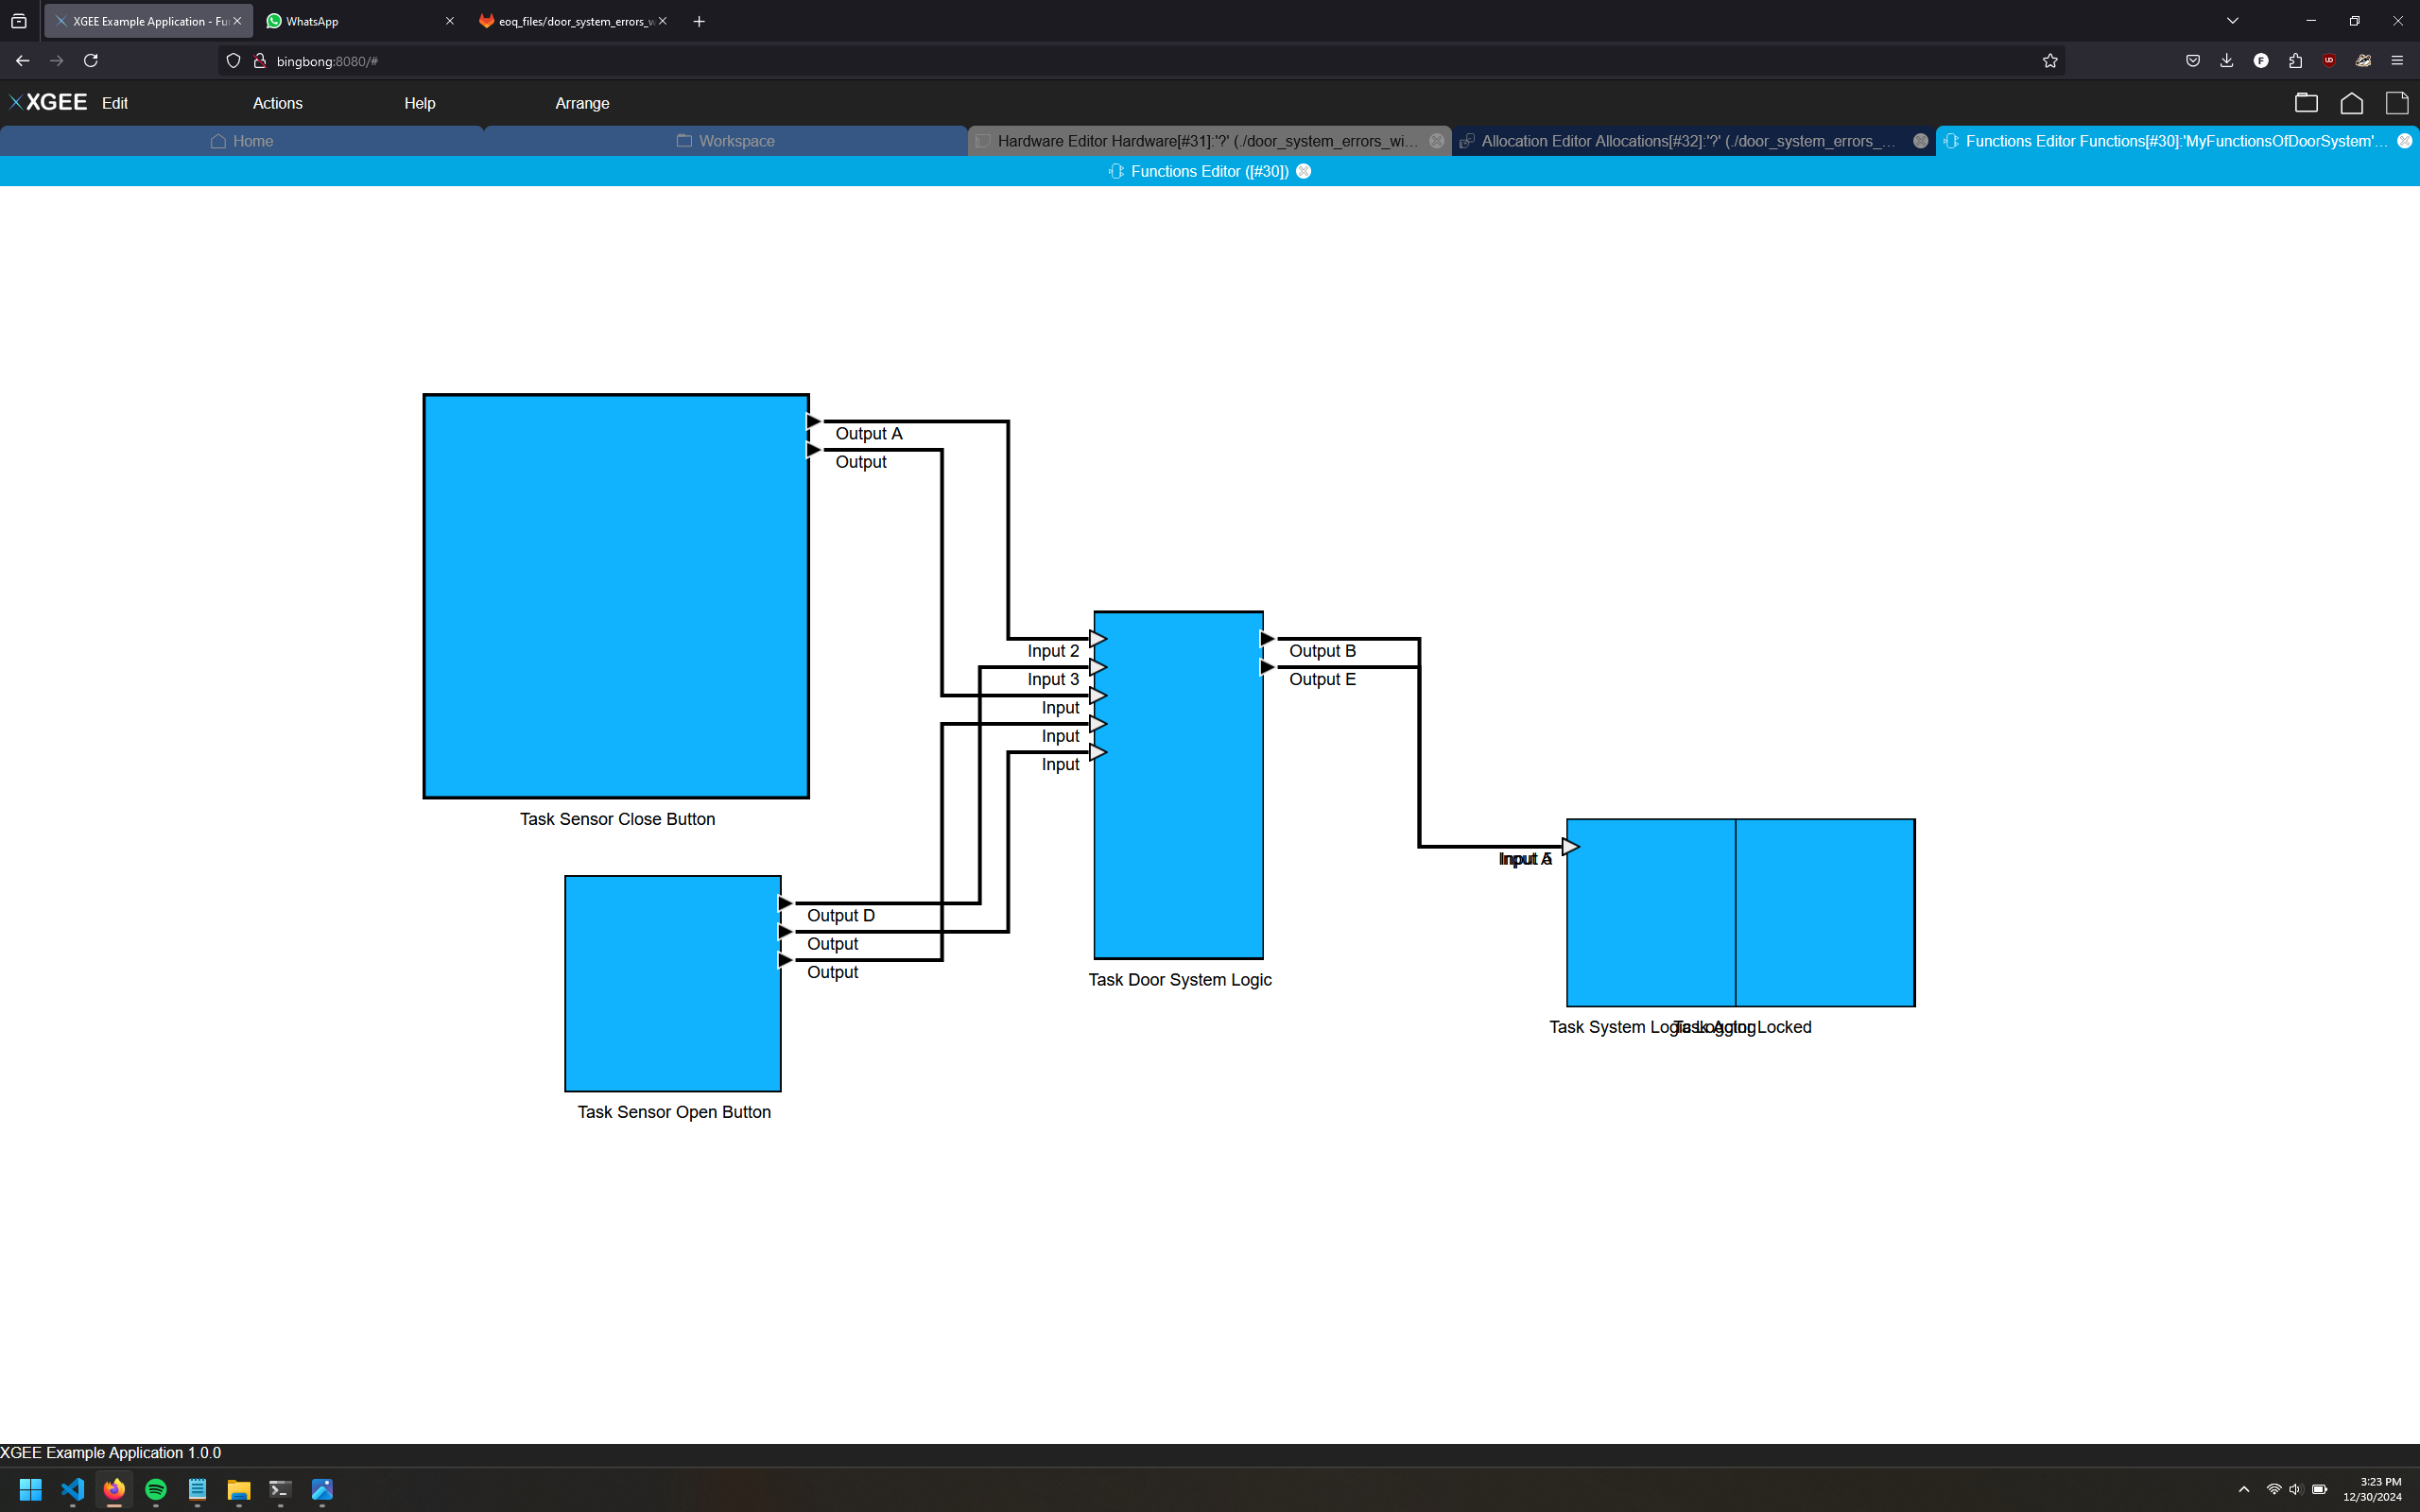
\includegraphics[width=0.9\textwidth]{images/vertices_too_close_to_each_other.png}
    \caption{Vertices too close to each other}
\end{figure}
\newpage

\section{Vertices overlapping}
\begin{figure}[H]
    \centering
    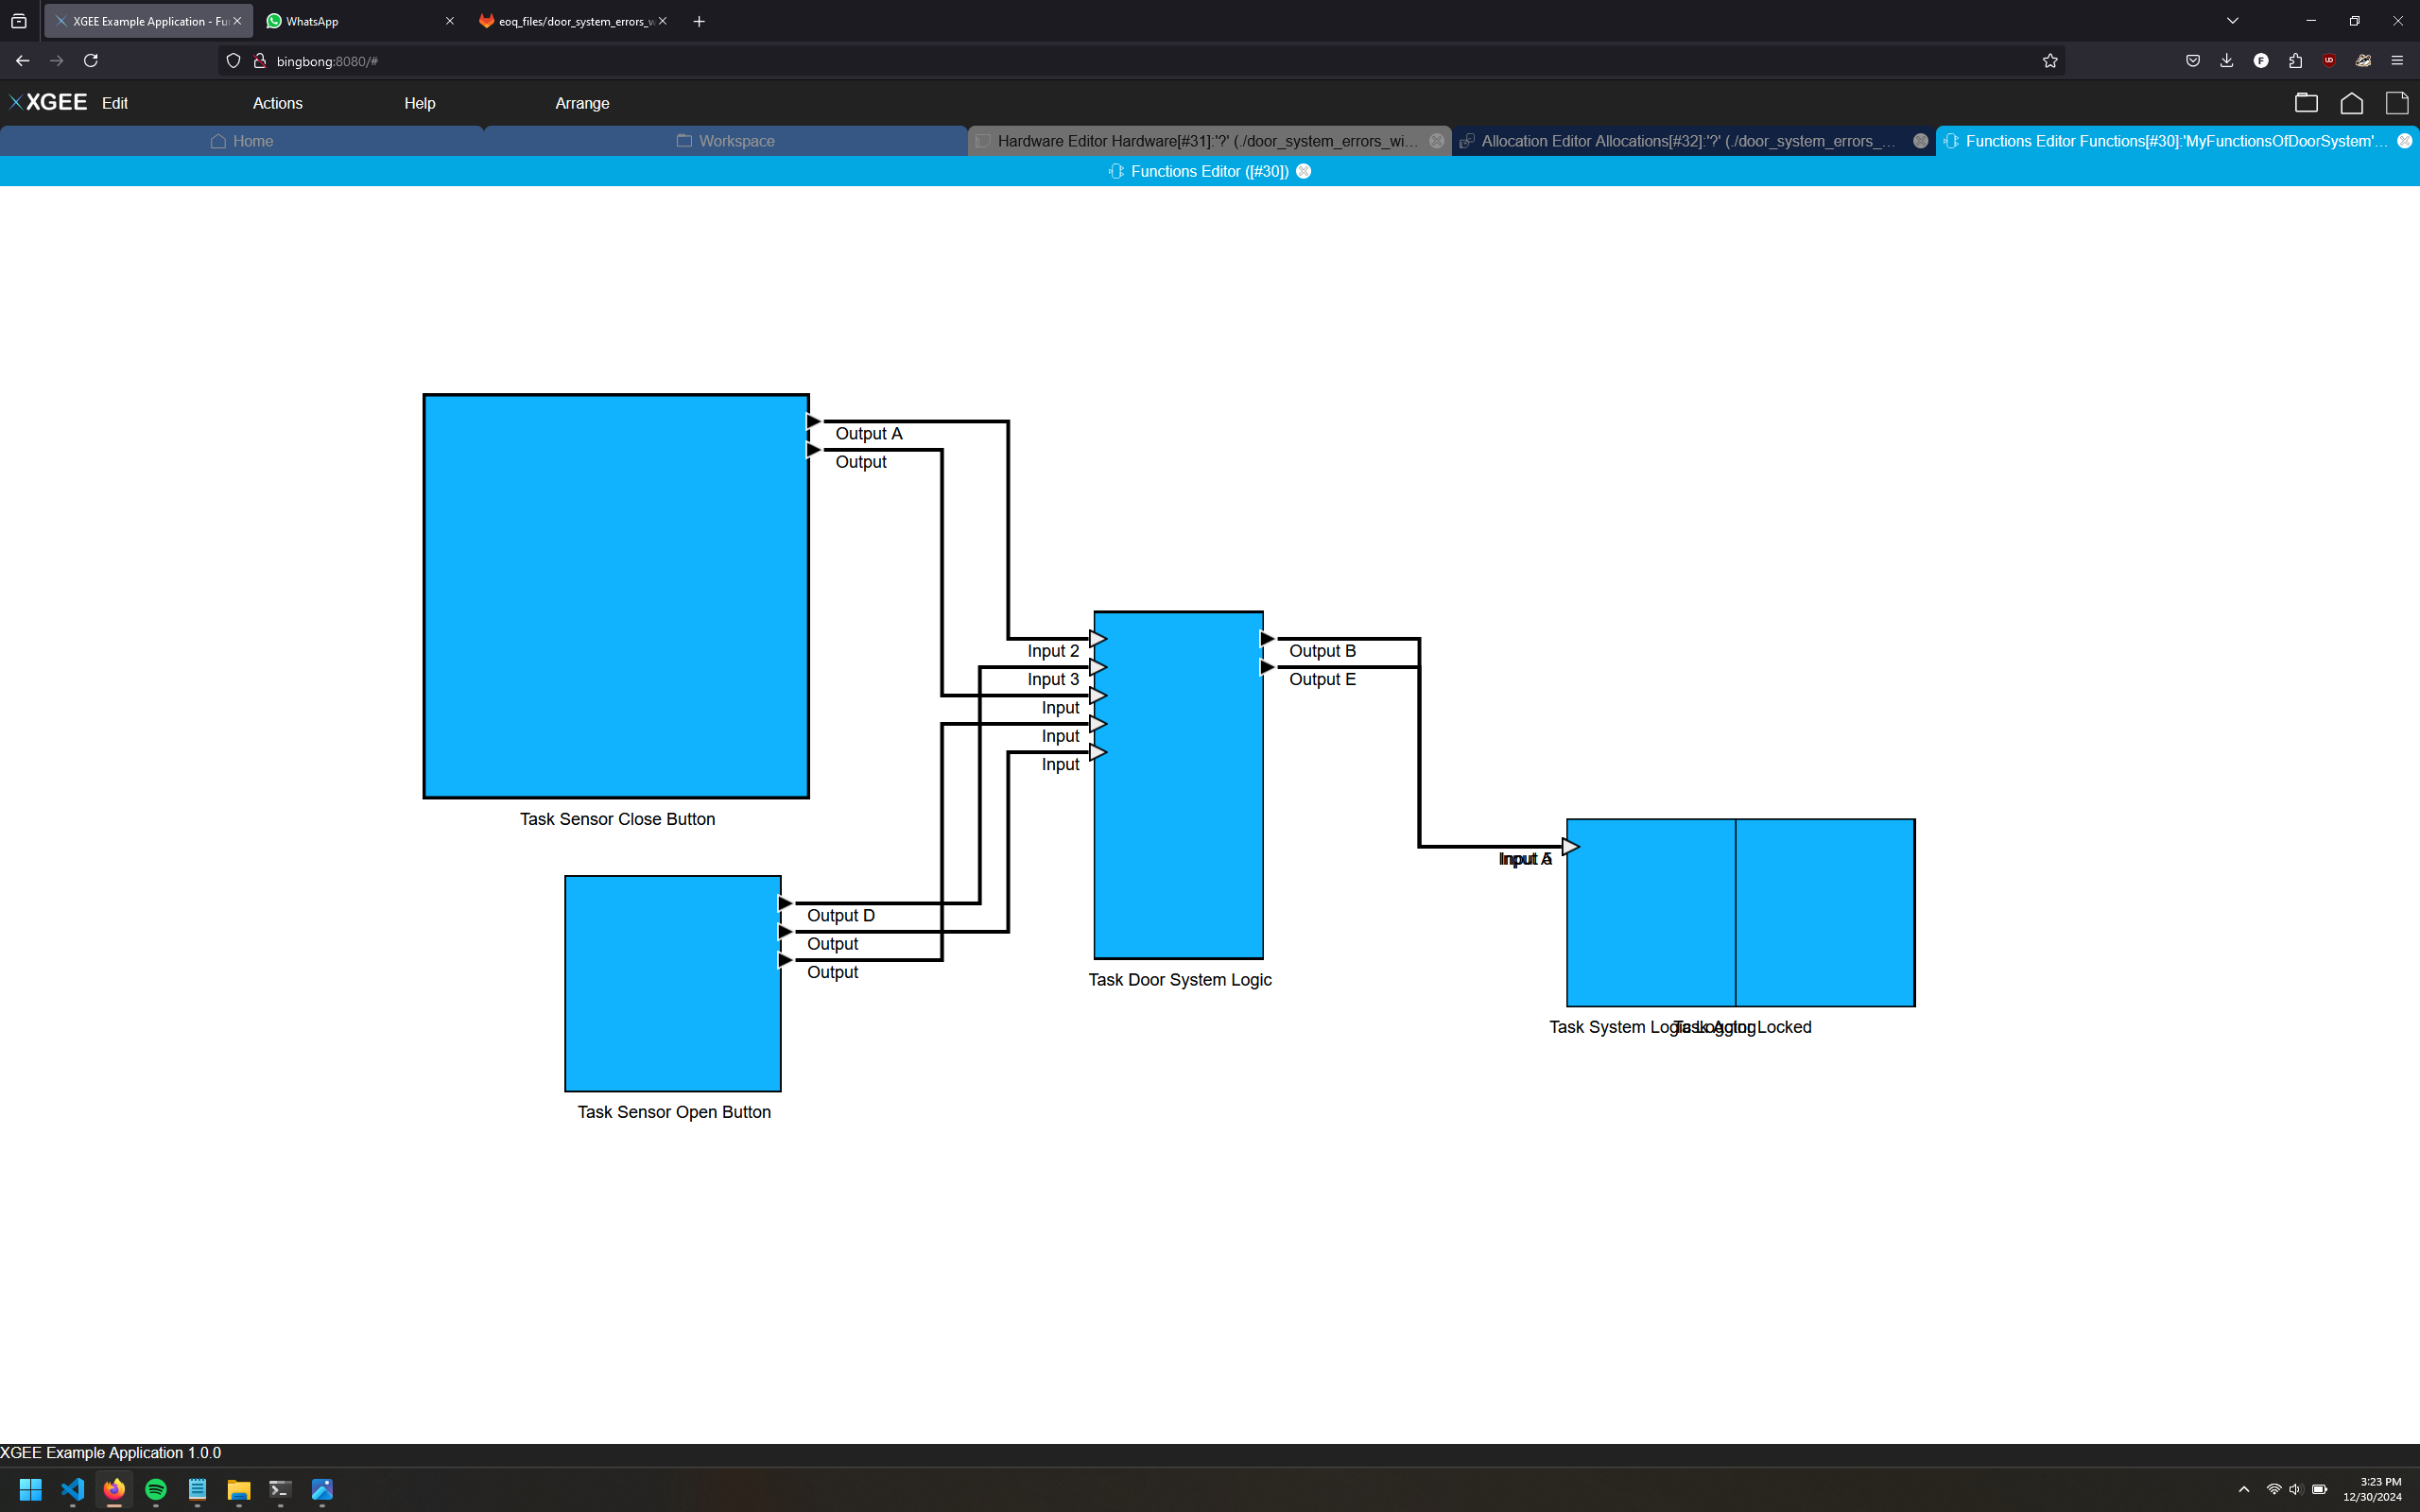
\includegraphics[width=0.9\textwidth]{images/vertices_too_close_to_each_other.png}
    \caption{Vertices overlapping}
\end{figure}
\newpage

\section{Vertices offscreen}
\begin{figure}[H]
    \centering
    % \includegraphics[width=0.9\textwidth]{images/vertices_offscreen.png}
    \caption{Vertices offscreen}
\end{figure}
\newpage

\section{Vertex without parent element}
\begin{figure}[H]
    \centering
    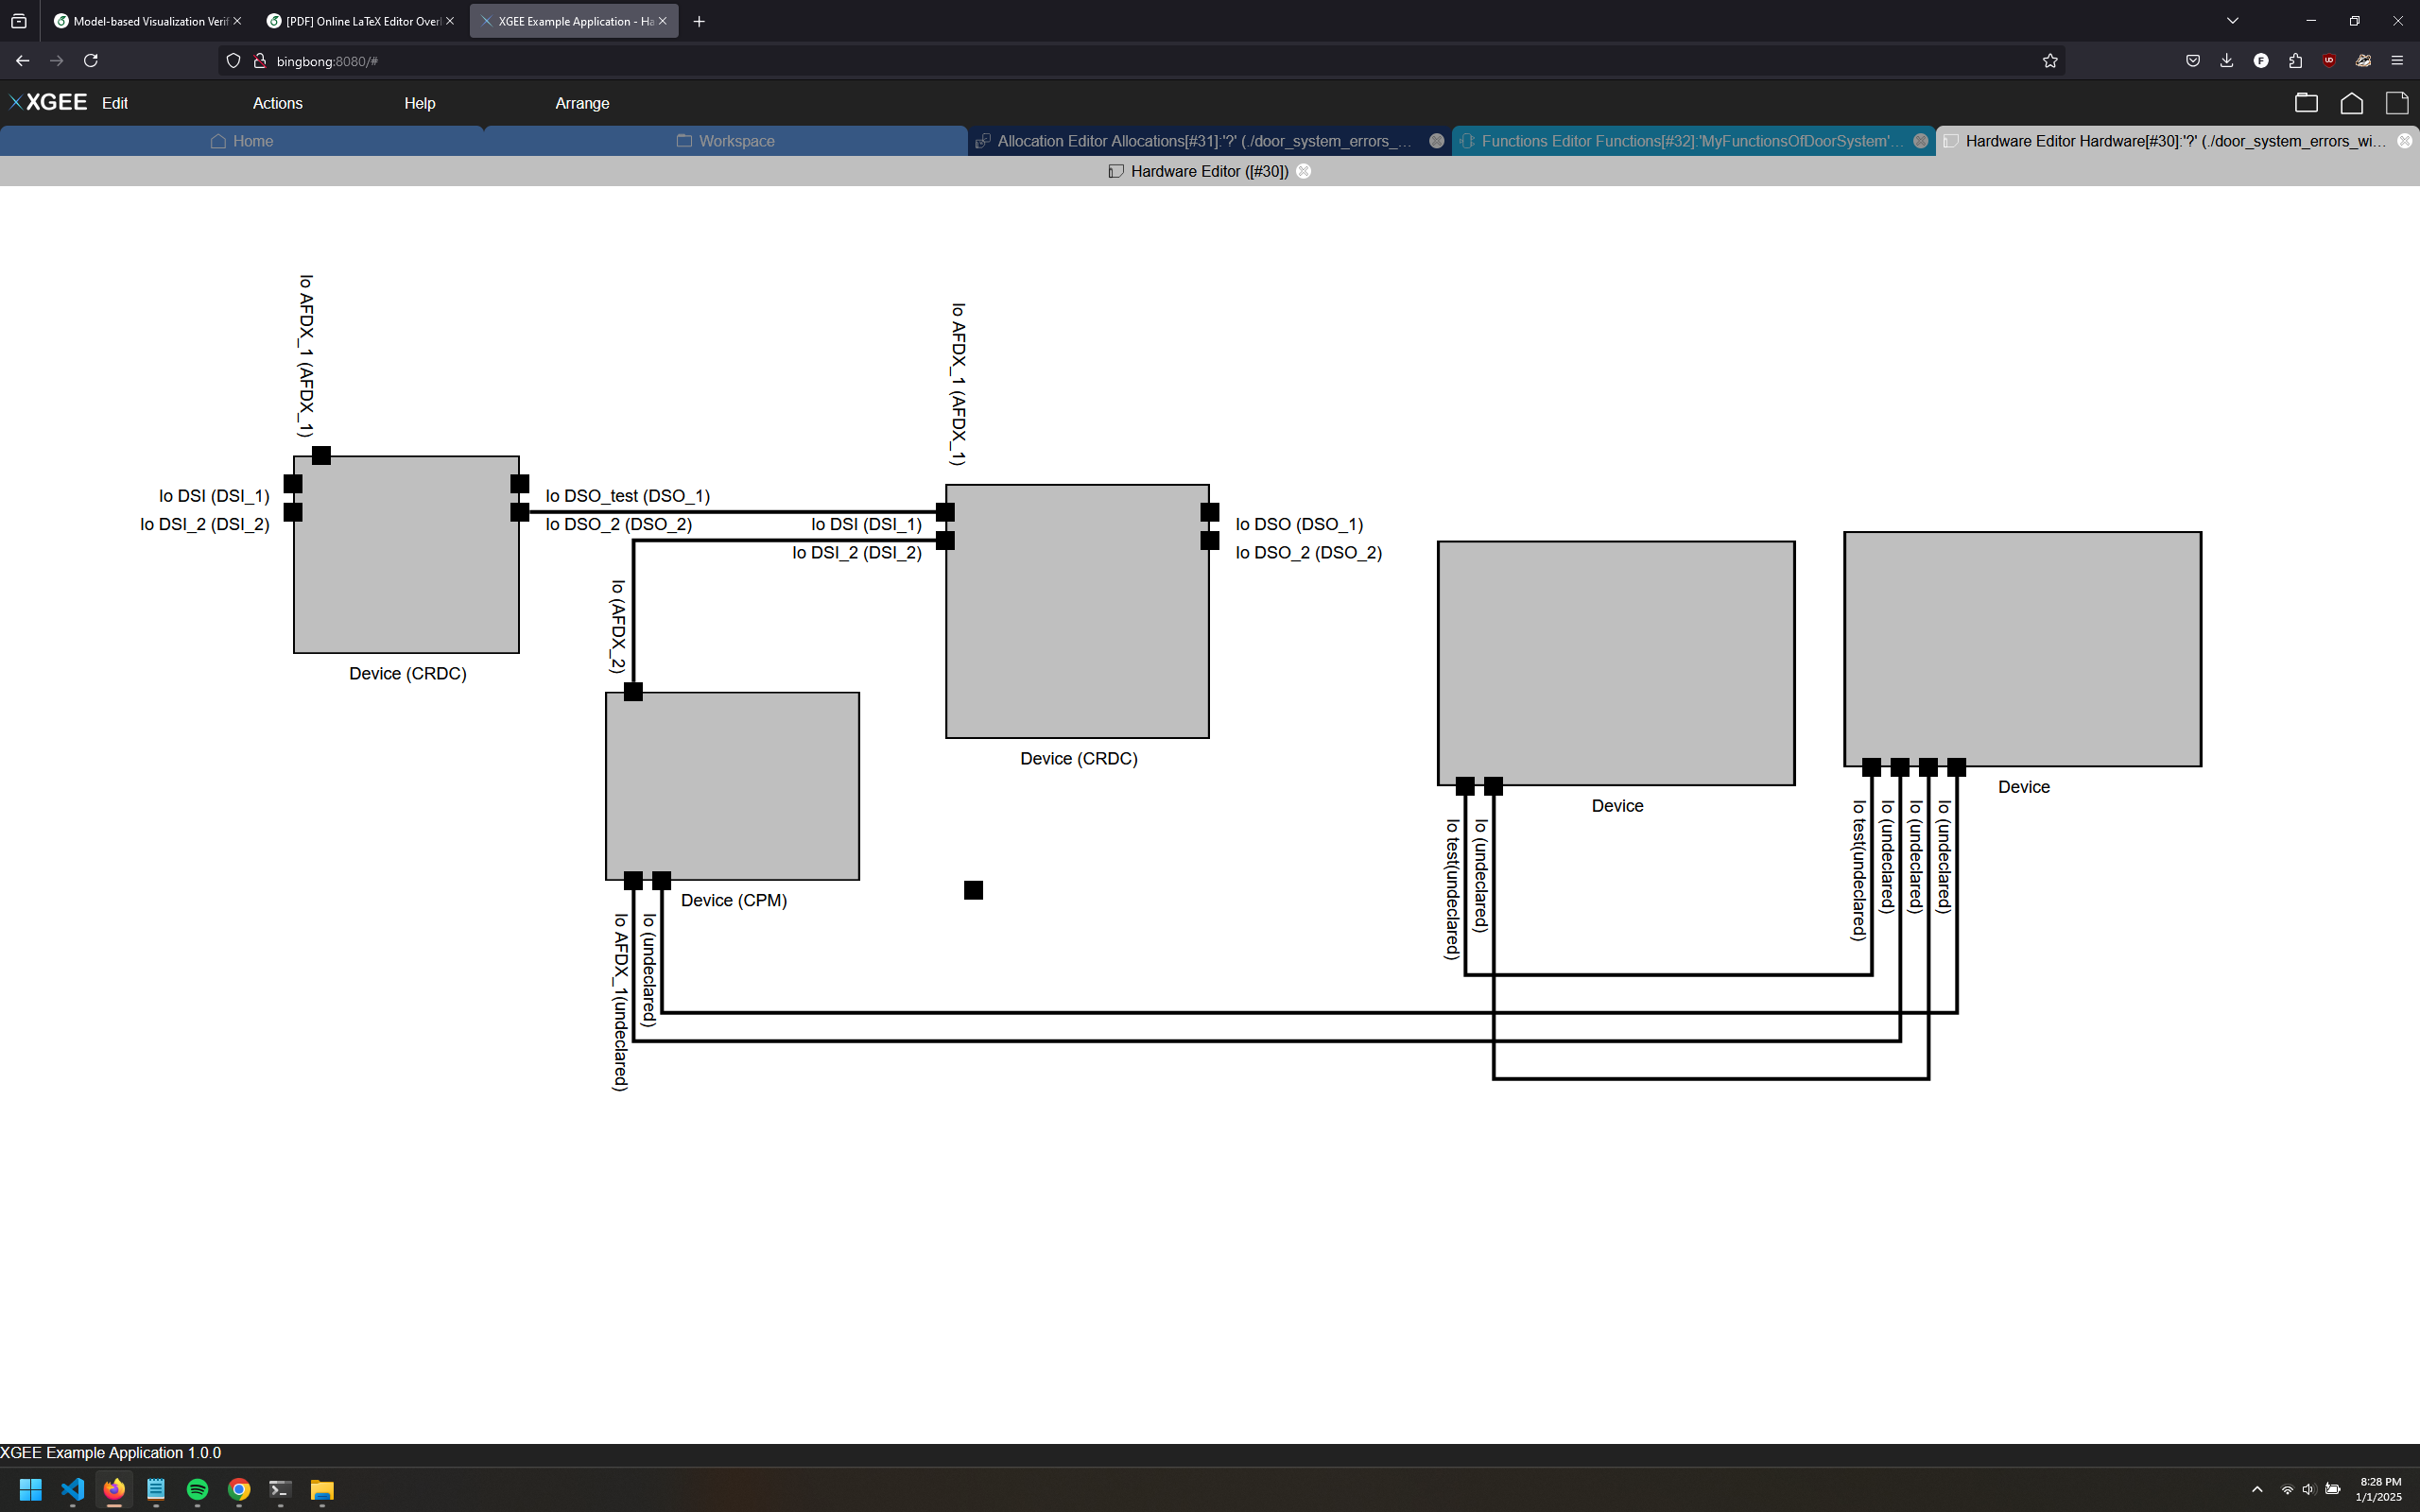
\includegraphics[width=0.9\textwidth]{images/vertex_without_parent_element.png}
    \caption{Vertex without parent element}
\end{figure}
\newpage

\section{Vertex displayed incorrectly}
\begin{figure}[H]
    \centering
    % \includegraphics[width=0.9\textwidth]{images/vertex_displayed_incorrectly.png}
    \caption{Vertex displayed incorrectly}
\end{figure}
\newpage

\section{Vertex in visualization, but not in model}
\begin{figure}[H]
    \centering
    % \includegraphics[width=0.9\textwidth]{images/vertex_in_visualization_but_not_in_model.png}
    \caption{Vertex in visualization, but not in model}
\end{figure}
\newpage

\section{Vertex in model, but not in visualization}
\begin{figure}[H]
    \centering
    % \includegraphics[width=0.9\textwidth]{images/vertex_in_model_but_not_in_visualization.png}
    \caption{Vertex in model, but not in visualization}
\end{figure}
\newpage

\section{Edge too thin}
\begin{figure}[H]
    \centering
    % \includegraphics[width=0.9\textwidth]{images/edge_too_thin.png}
    \caption{Edge too thin}
\end{figure}
\newpage

\section{Edge too wide}
\begin{figure}[H]
    \centering
    % \includegraphics[width=0.9\textwidth]{images/edge_too_wide.png}
    \caption{Edge too wide}
\end{figure}
\newpage

\section{Edge wrong color}
\begin{figure}[H]
    \centering
    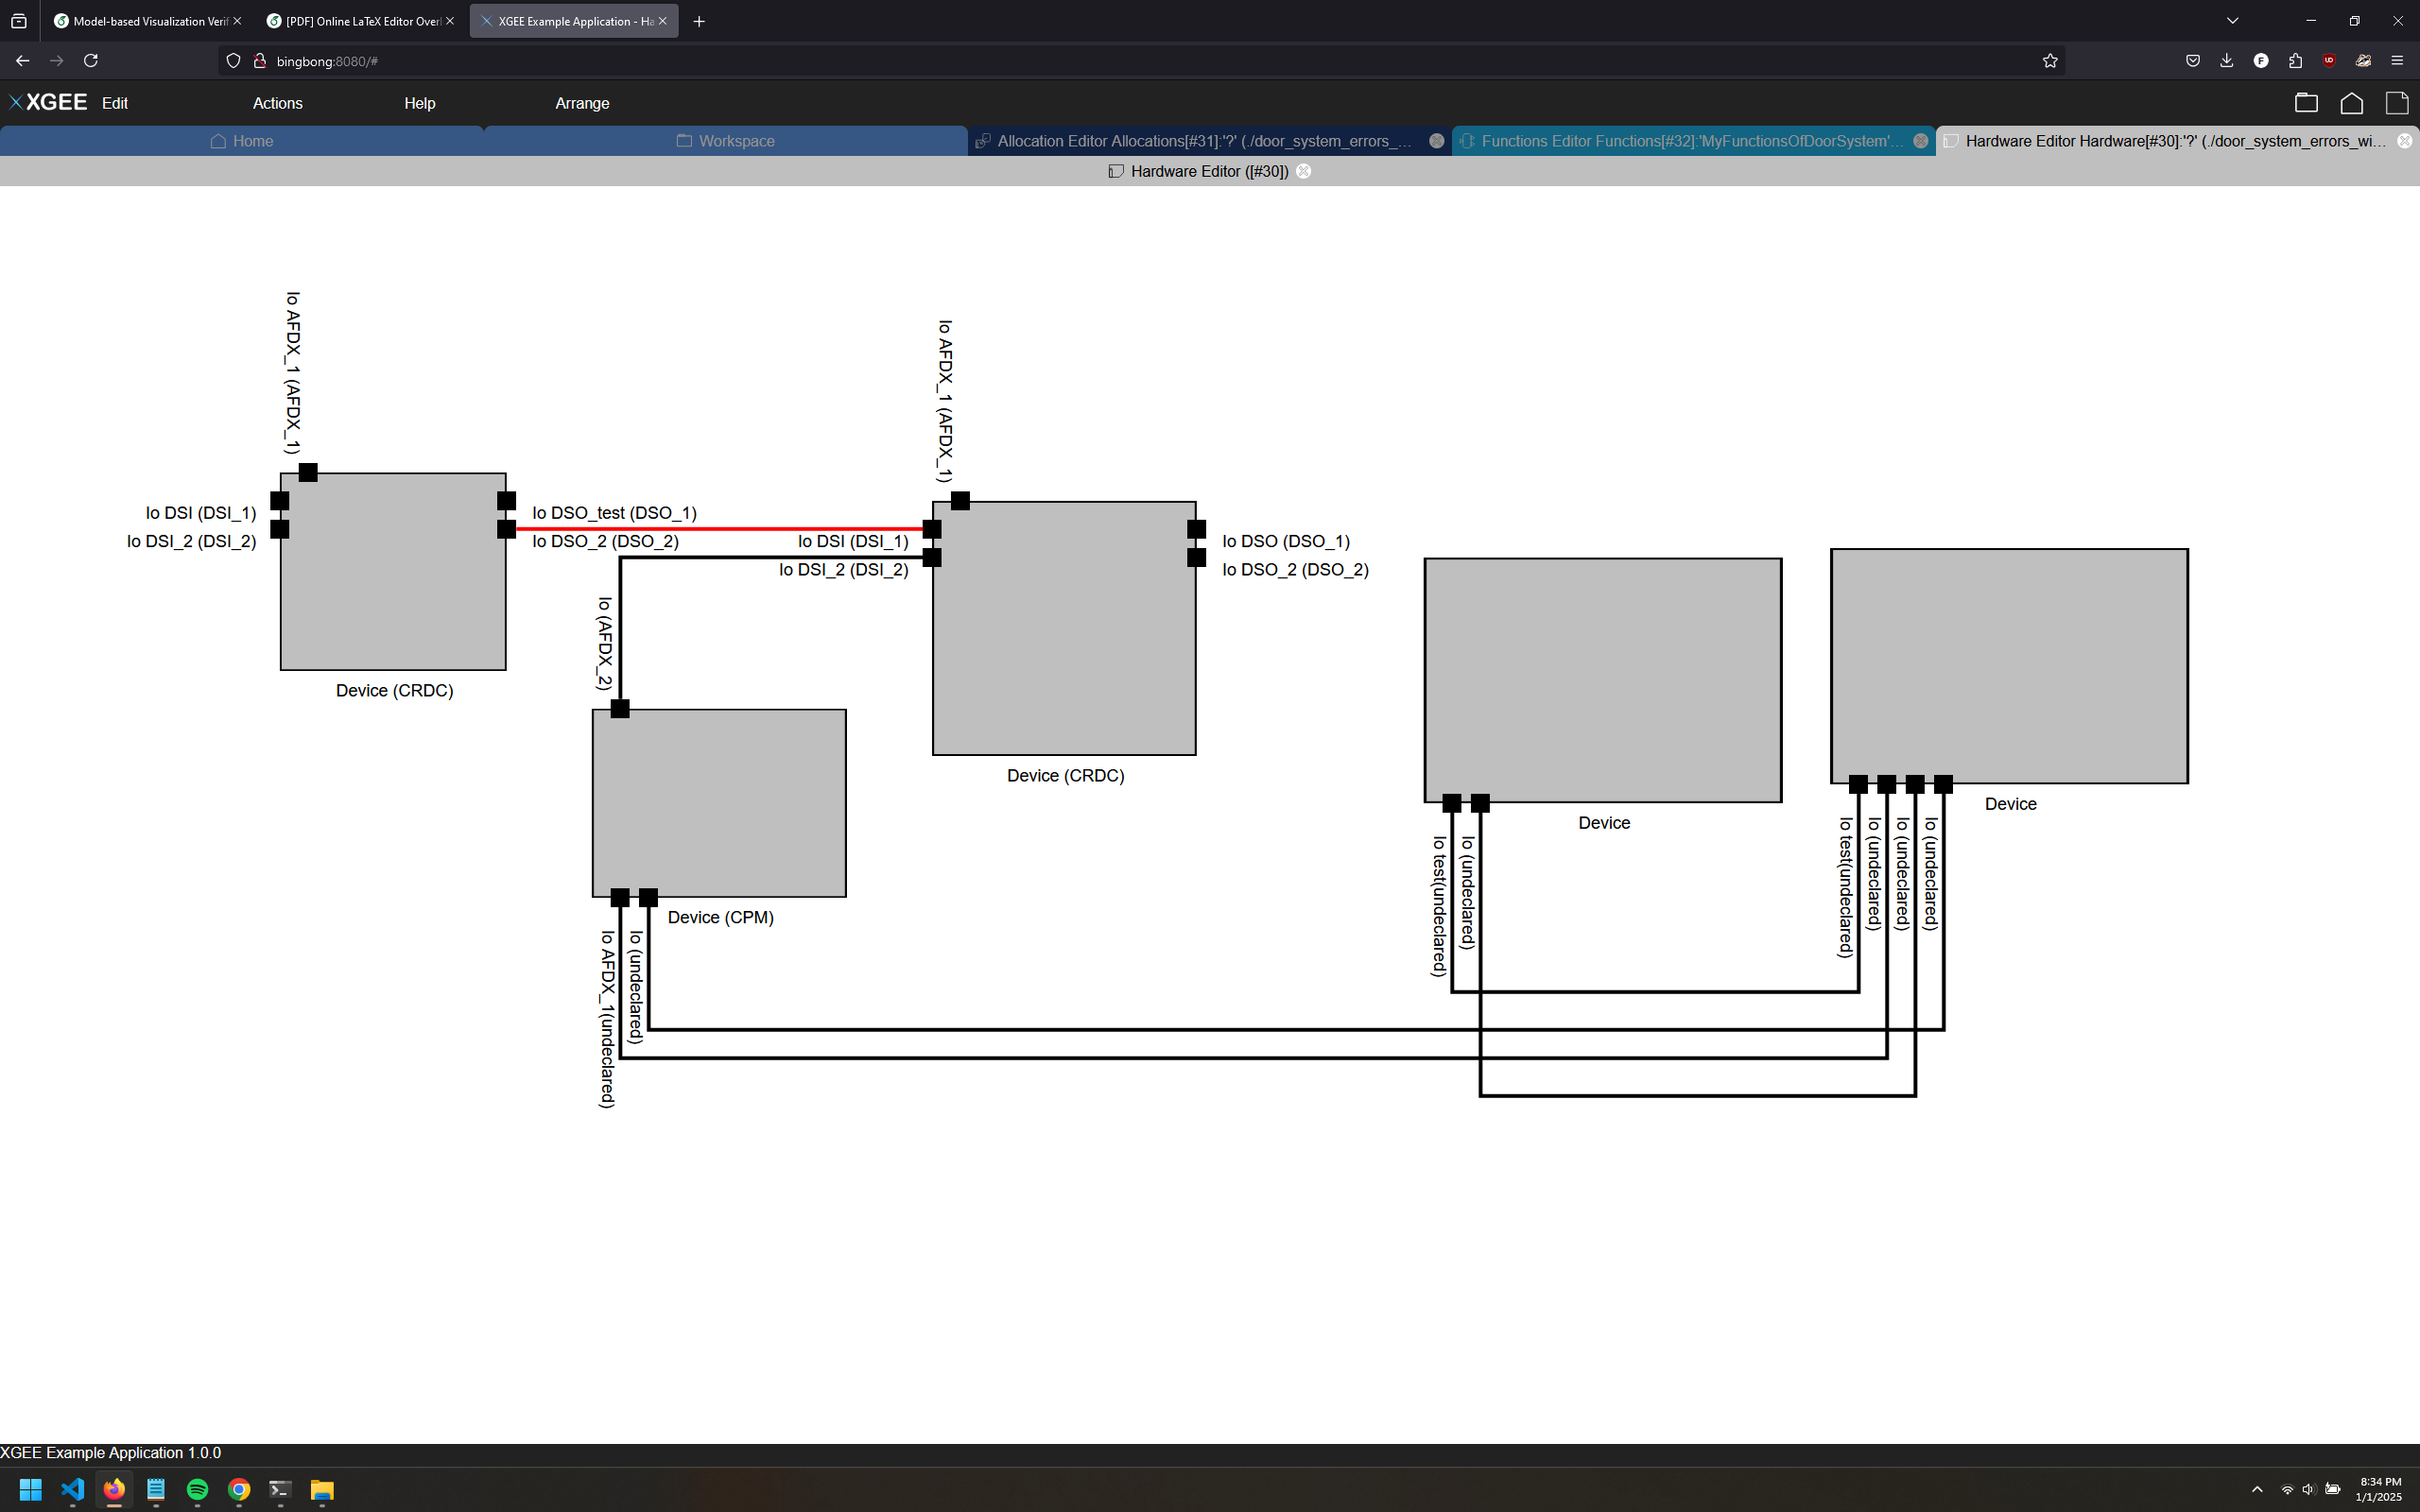
\includegraphics[width=0.9\textwidth]{images/edge_wrong_color.png}
    \caption{Edge wrong color}
\end{figure}
\newpage

\section{Edge not connected to anything}
\begin{figure}[H]
    \centering
    % \includegraphics[width=0.9\textwidth]{images/edge_not_connected_to_anything.png}
    \caption{Edge not connected to anything}
\end{figure}
\newpage

\section{Edge connecting wrong elements}
\begin{figure}[H]
    \centering
    % \includegraphics[width=0.9\textwidth]{images/edge_connecting_wrong_elements.png}
    \caption{Edge connecting wrong elements}
\end{figure}
\newpage

\section{Edges too close to each other}
\begin{figure}[H]
    \centering
    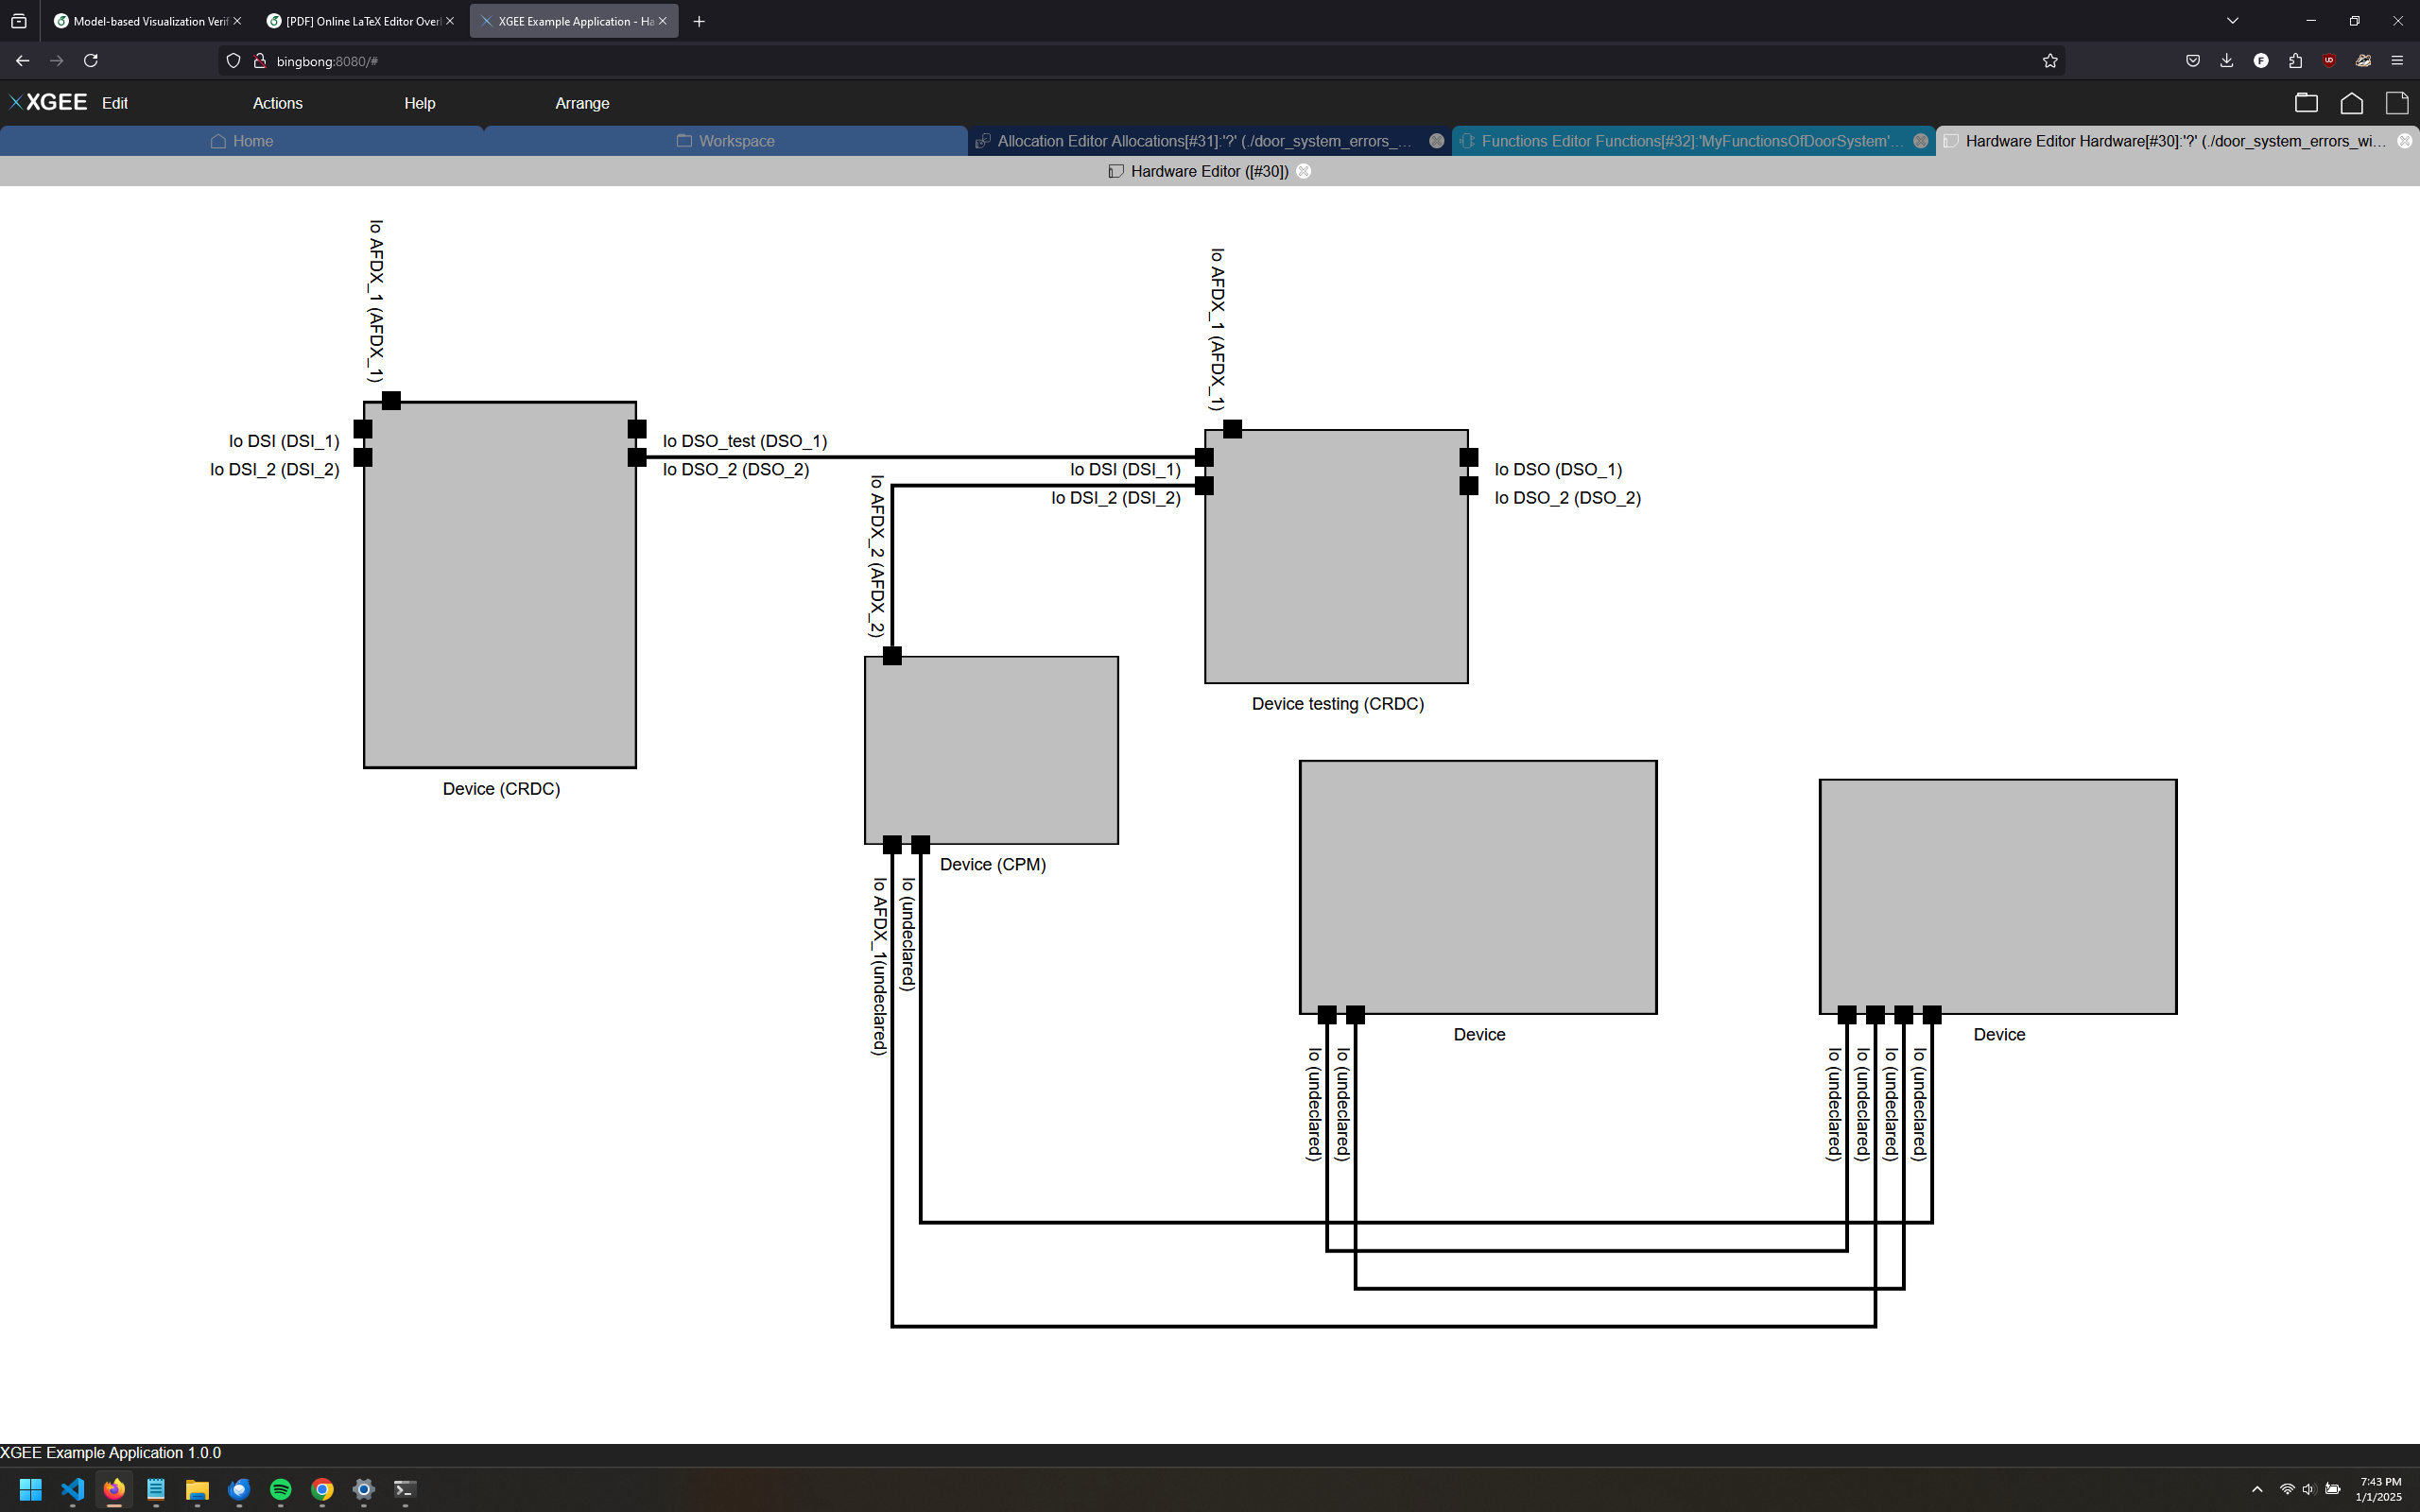
\includegraphics[width=0.9\textwidth]{images/edges_too_close_to_each_other.png}
    \caption{Edges too close to each other}
\end{figure}
\newpage

\section{Edges forming ambigous intersections}
\begin{figure}[H]
    \centering
    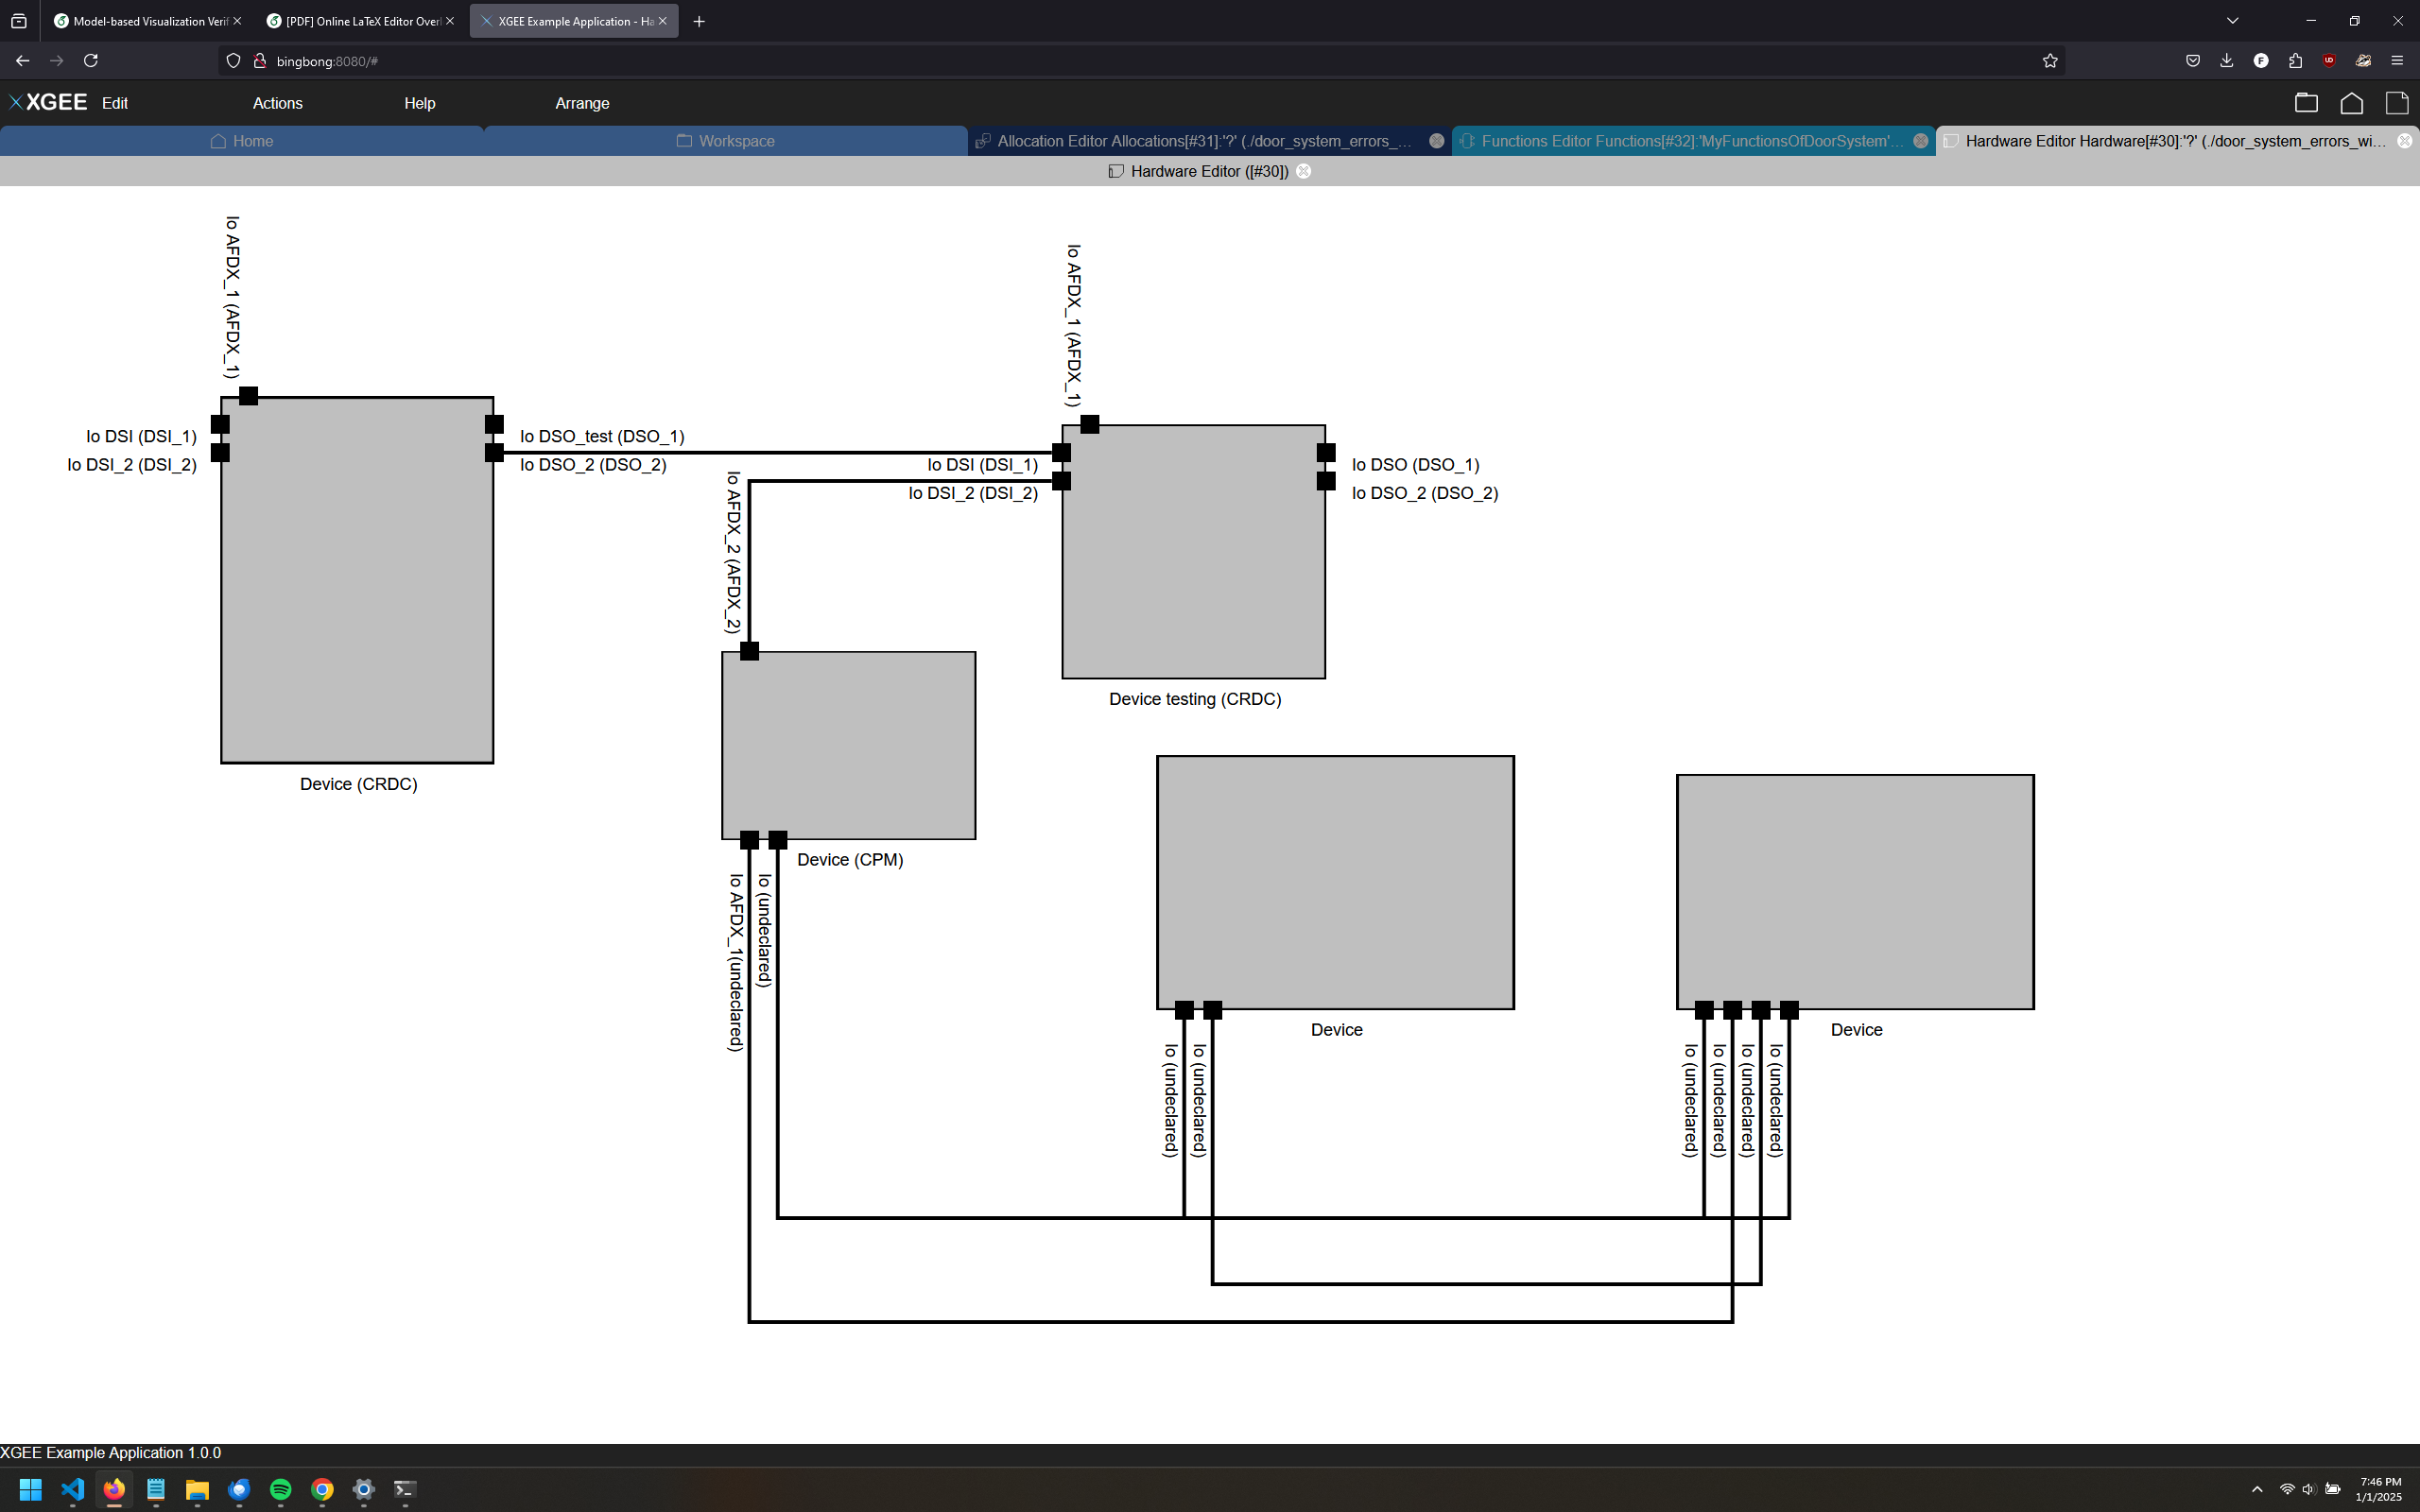
\includegraphics[width=0.9\textwidth]{images/edges_forming_ambigous_intersections.png}
    \caption{Edges forming ambigous intersections}
\end{figure}
\newpage

\section{Edges offscreen}
\begin{figure}[H]
    \centering
    % \includegraphics[width=0.9\textwidth]{images/edges_offscreen.png}
    \caption{Edges offscreen}
\end{figure}
\newpage

\section{Edge in visualization, but not in model}
\begin{figure}[H]
    \centering
    % \includegraphics[width=0.9\textwidth]{images/edge_in_visualization_but_not_in_model.png}
    \caption{Edge in visualization, but not in model}
\end{figure}
\newpage

\section{Edge in model, but not in visualization}
\begin{figure}[H]
    \centering
    % \includegraphics[width=0.9\textwidth]{images/edge_in_model_but_not_in_visualization.png}
    \caption{Edge in model, but not in visualization}
\end{figure}
\newpage

\section{Text too small}
\begin{figure}[H]
    \centering
    % \includegraphics[width=0.9\textwidth]{images/text_too_small.png}
    \caption{Text too small}
\end{figure}
\newpage

\section{Text too large}
\begin{figure}[H]
    \centering
    % \includegraphics[width=0.9\textwidth]{images/text_too_large.png}
    \caption{Text too large}
\end{figure}
\newpage

\section{Text wrong color}
\begin{figure}[H]
    \centering
    % \includegraphics[width=0.9\textwidth]{images/text_wrong_color.png}
    \caption{Text wrong color}
\end{figure}
\newpage

\section{Text in wrong position relative to parent element}
\begin{figure}[H]
    \centering
    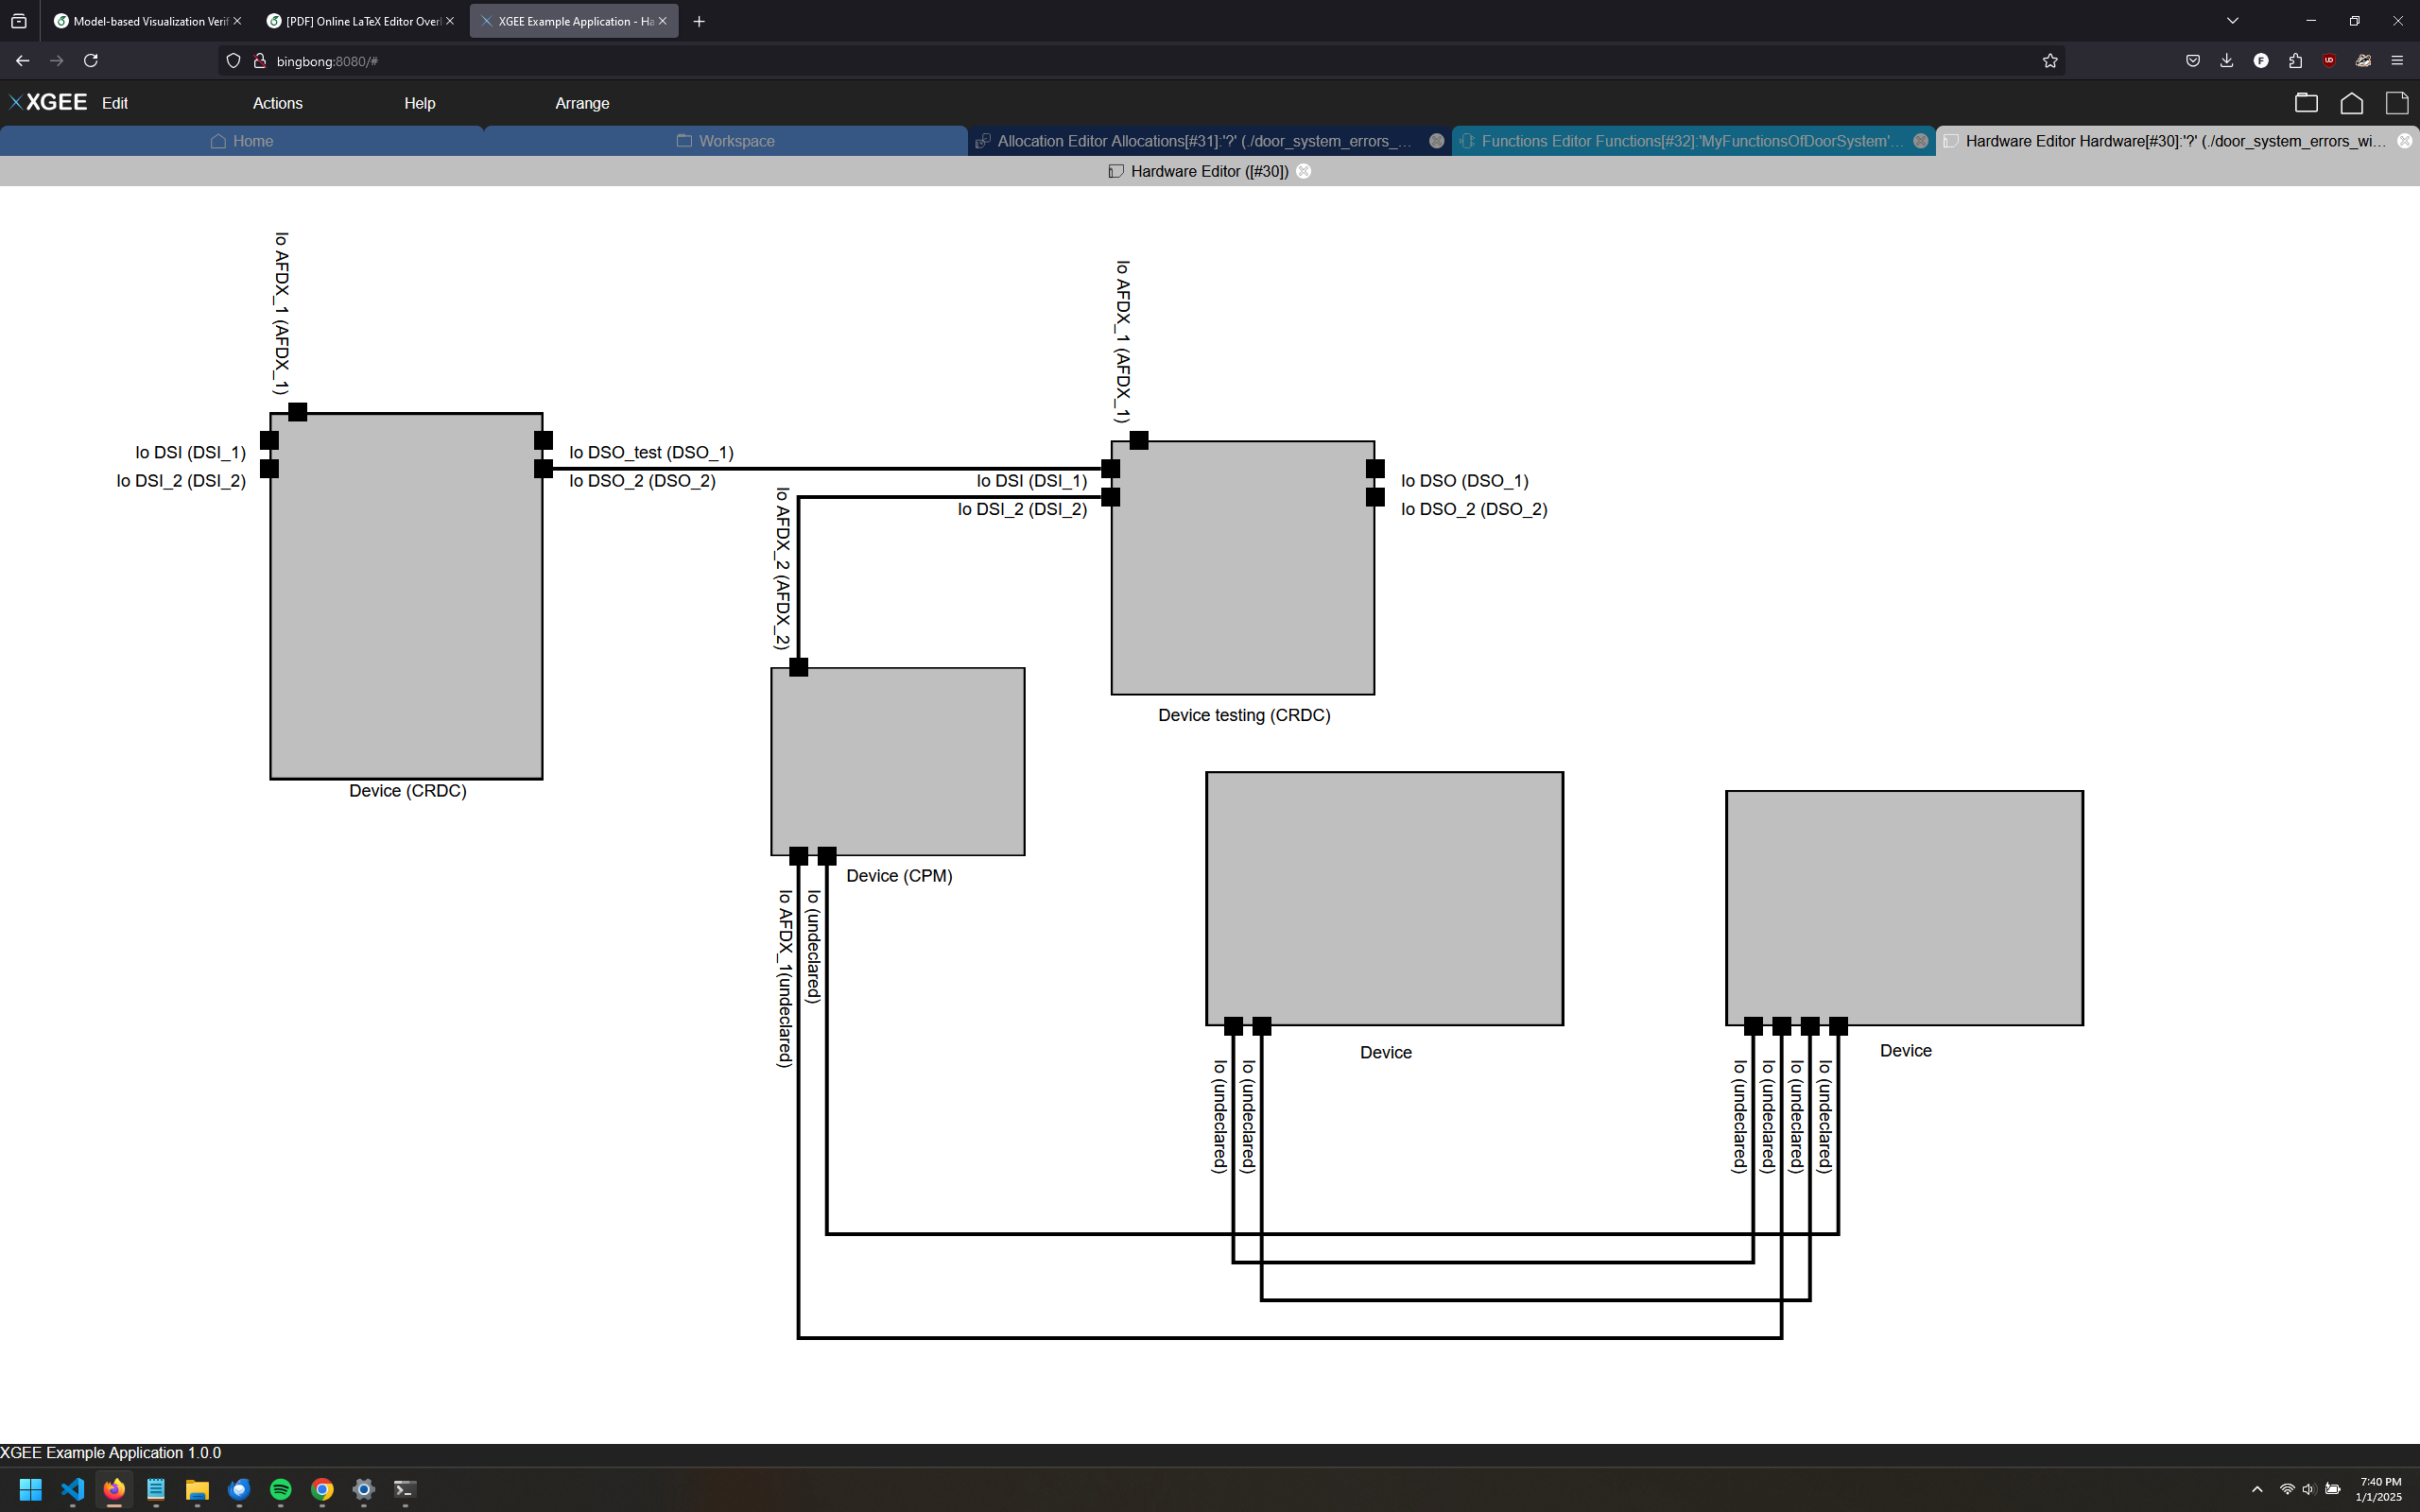
\includegraphics[width=0.9\textwidth]{images/text_in_wrong_position_relative_to_parent_element.png}
    \caption{Text in wrong position relative to parent element}
\end{figure}
\newpage

\section{Text without parent element}
\begin{figure}[H]
    \centering
    % \includegraphics[width=0.9\textwidth]{images/text_without_parent_element.png}
    \caption{Text without parent element}
\end{figure}
\newpage

\section{Texts too close to each other}
\begin{figure}[H]
    \centering
    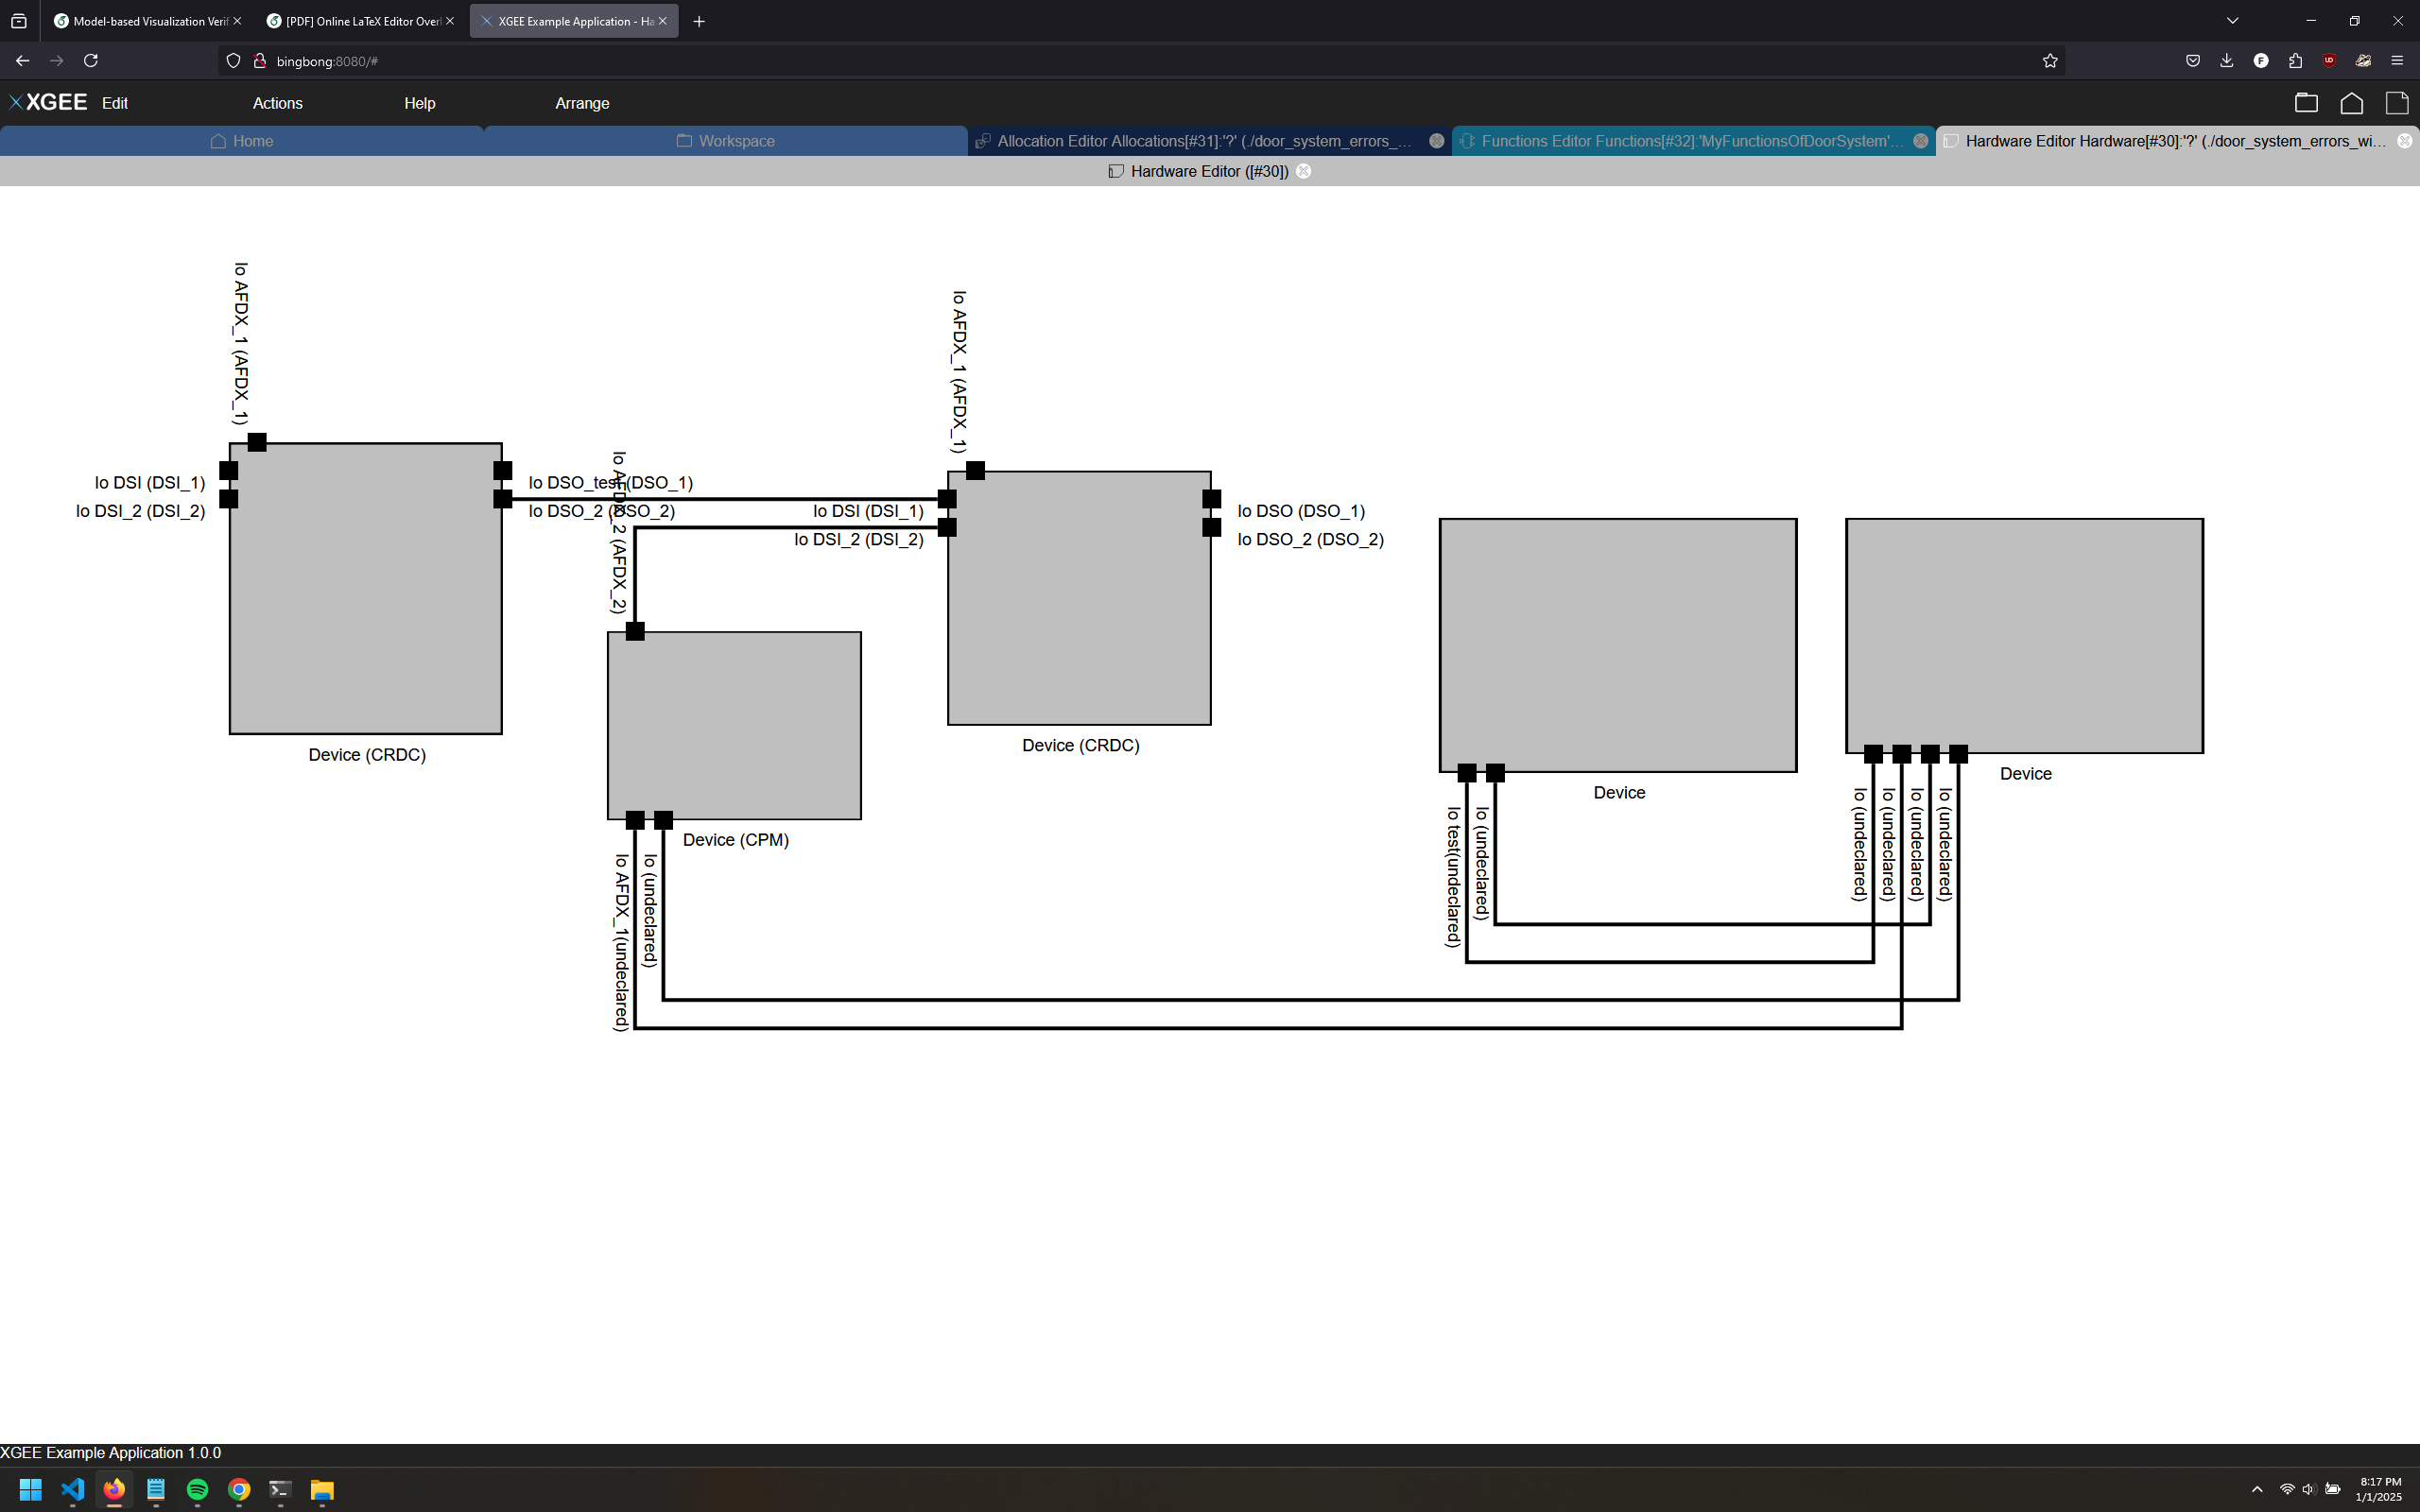
\includegraphics[width=0.9\textwidth]{images/texts_too_close_to_each_other.png}
    \caption{Texts too close to each other}
\end{figure}
\newpage

\section{Texts overlapping}
\begin{figure}[H]
    \centering
    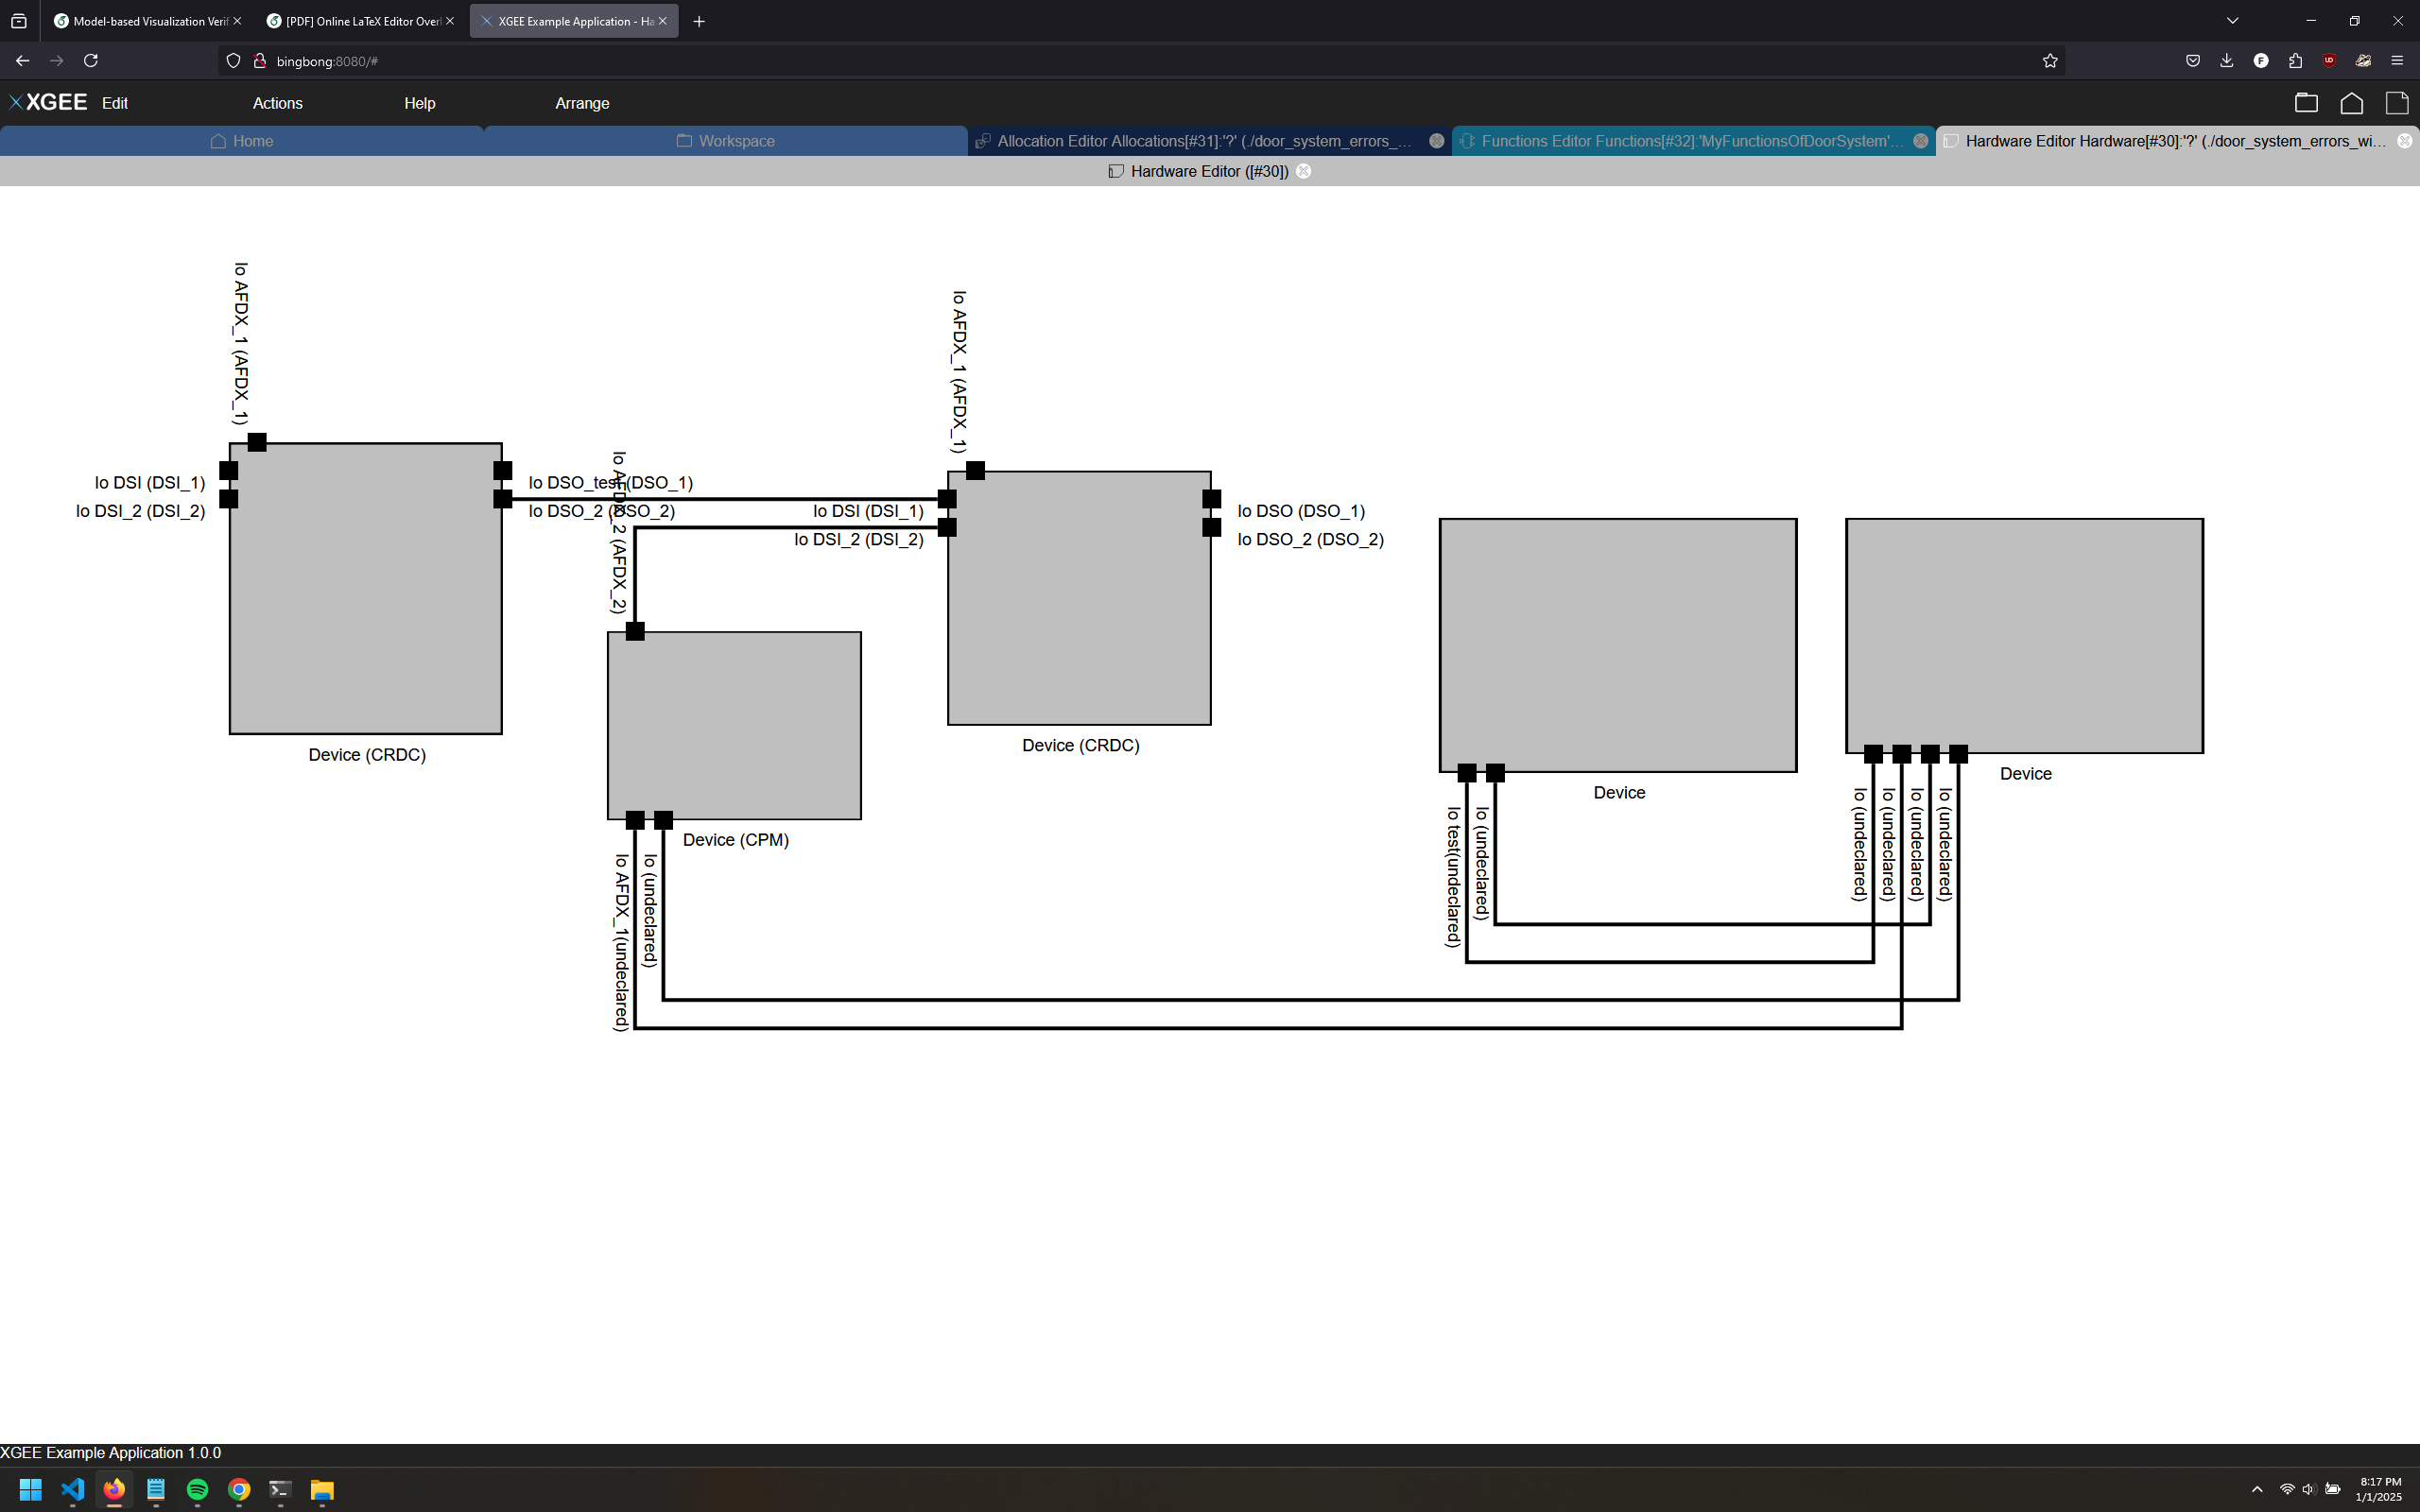
\includegraphics[width=0.9\textwidth]{images/texts_too_close_to_each_other.png}
    \caption{Texts overlapping}
\end{figure}
\newpage

\section{Text overlapping with other elements}
\begin{figure}[H]
    \centering
    % \includegraphics[width=0.9\textwidth]{images/text_overlapping_with_other_elements.png}
    \caption{Text overlapping with other elements}
\end{figure}
\newpage

\section{Text offscreen}
\begin{figure}[H]
    \centering
    % \includegraphics[width=0.9\textwidth]{images/text_offscreen.png}
    \caption{Text offscreen}
\end{figure}
\newpage

\section{Text in visualization, but not in model}
\begin{figure}[H]
    \centering
    % \includegraphics[width=0.9\textwidth]{images/text_in_visualization_but_not_in_model.png}
    \caption{Text in visualization, but not in model}
\end{figure}
\newpage

\section{Text in model, but not in visualization}
\begin{figure}[H]
    \centering
    % \includegraphics[width=0.9\textwidth]{images/text_in_model_but_not_in_visualization.png}
    \caption{Text in model, but not in visualization}
\end{figure}
\newpage

\section{Text wrong in visualization}
\begin{figure}[H]
    \centering
    % \includegraphics[width=0.9\textwidth]{images/text_wrong_in_visualization.png}
    \caption{Text wrong in visualization}
\end{figure}
\newpage

\end{document}
